\documentclass[conference]{IEEEtran}
\IEEEoverridecommandlockouts
% The preceding line is only needed to identify funding in the first footnote. If that is unneeded, please comment it out.
\usepackage{cite}
\usepackage{amsmath,amssymb,amsfonts}
\usepackage{algorithm}
\usepackage{algorithmic}
\usepackage{graphicx}
\usepackage{textcomp}
\usepackage{xcolor}
\usepackage{booktabs}
\usepackage{multirow}
\usepackage{array}
\usepackage{url}
\usepackage{balance}

\def\BibTeX{{\rm B\kern-.05em{\sc i\kern-.025em b}\kern-.08em
    T\kern-.1667em\lower.7ex\hbox{E}\kern-.125emX}}

\begin{document}

\title{Fused Kolmogorov-Arnold Network and Bidirectional Gated Recurrent Units (KAN-GRU) for Multi-Label V2X Message Classification and Threat Intelligence}

\author{
\IEEEauthorblockN{Pratyaksh Manav}
\IEEEauthorblockA{\textit{Bachelor of Technology in} \\
\textit{Computer Science \& Engineering} \\
\textit{Specialization in AI} \\
\textit{School of Computer Science \& Tech.} \\
\textit{Bennett University} \\
Greater Noida, India \\
manavpratyaksh@gmail.com}
\and
\IEEEauthorblockN{Abhayraj Verma}
\IEEEauthorblockA{\textit{Bachelor of Technology in} \\
\textit{Computer Science \& Engineering} \\
\textit{Specialization in AI} \\
\textit{School of Computer Science \& Tech.} \\
\textit{Bennett University} \\
Greater Noida, India}
\and
\IEEEauthorblockN{Arnav Tomar}
\IEEEauthorblockA{\textit{Bachelor of Technology in} \\
\textit{Computer Science \& Engineering} \\
\textit{Specialization in AI} \\
\textit{School of Computer Science \& Tech.} \\
\textit{Bennett University} \\
Greater Noida, India}
}

\maketitle

\begin{abstract}
Connected and Autonomous Vehicles (CAVs) rely fundamentally on Vehicle-to-Everything (V2X) wireless communications to disseminate mission-critical traffic safety telemetry and coordinate distributed collision avoidance maneuvers. Standardized communication frameworks, such as Dedicated Short-Range Communications (DSRC / IEEE 802.11p) and Cellular V2X (3GPP C-V2X / 5G NR-V2X), facilitate millisecond-level telemetry exchange. However, the decentralized, open-access wireless medium renders vehicular networks acutely susceptible to sophisticated cyber-physical intrusions, including Sybil identity fabrication, kinematic GPS coordinate tampering, message replay attacks, and fraudulent hazard dissemination. Existing Intrusion Detection Systems (IDS) frequently struggle to resolve complex non-linear attribute dependencies and sequential temporal patterns from variable-length message payloads, resulting in elevated false alarm rates and degraded multi-label classification accuracy. In this work, we propose a novel deep learning framework that fuses Kolmogorov-Arnold Networks (KAN) with Bidirectional Gated Recurrent Units (BiGRU), augmented by a trainable self-attention pooling mechanism, designated as \textbf{KAN-GRU}. Operating on standardized IEEE DataPort V2X message payloads (BSM, CAM, DENM, SPAT, MAP, and RSA), the proposed architecture incorporates an enhanced preprocessing pipeline utilizing sub-token feature extraction, sequence post-padding, and dense embedding vectorization. The KAN layers employ learnable B-spline and SiLU edge activation functions to model complex non-linear telemetry interactions, while the BiGRU captures forward and backward temporal dependencies. Benchmarked against baseline architectures from IEEE Document 11308890 (BRNN, CNN-BRNN, BLSTM, and CNN-BLSTM) as well as standalone KAN and GRU models across 6,000 empirical instances, the proposed KAN-GRU model achieves state-of-the-art performance with an accuracy of \textbf{97.80\%}, precision of \textbf{99.45\%}, recall of \textbf{96.80\%}, F1-score of \textbf{98.10\%}, and loss of \textbf{0.14}, substantially outperforming the original baseline CNN-BRNN benchmark (90.00\% accuracy) while guaranteeing an end-to-end inference latency under 8.5 milliseconds.
\end{abstract}

\begin{IEEEkeywords}
Vehicle-to-Everything (V2X), Kolmogorov-Arnold Networks (KAN), Gated Recurrent Units (GRU), Multi-Label Classification, Intrusion Detection System (IDS), Deep Learning, Cyber-Physical Systems.
\end{IEEEkeywords}

\section{Introduction}
Intelligent Transportation Systems (ITS) and Cooperative Connected and Autonomous Vehicles (CAVs) have experienced rapid technological evolution over the past decade, transforming modern transportation into an interconnected cyber-physical paradigm \cite{tabaa2020green, saurabh2022lbdmids}. At the cornerstone of this autonomous ecosystem lies Vehicle-to-Everything (V2X) communication, encompassing Vehicle-to-Vehicle (V2V), Vehicle-to-Infrastructure (V2I), Vehicle-to-Pedestrian (V2P), and Vehicle-to-Network (V2N) communication links standardized by the Society of Automotive Engineers (SAE J2735) and the European Telecommunications Standards Institute (ETSI ITS-G5) \cite{pourrahmani2022applications, rejeb2023unleashing}. Through periodic high-frequency broadcasts and event-triggered safety notifications, vehicular nodes continuously disseminate kinematic state vectors, environmental hazard alerts, and intersection topologies, providing vehicles with omnidirectional perception that extends far beyond the physical range of onboard LiDAR, RADAR, and optical camera sensors.

\subsection{V2X Ecosystem and Communication Architecture}
The foundational architecture and operational communication modes governing autonomous and connected vehicular environments are illustrated in Fig. \ref{fig:ecosystem}. The modern V2X vehicular ecosystem comprises four foundational operational nodes:
\begin{enumerate}
    \item \textbf{On-Board Unit (OBU)}: Modern vehicular transceivers embedded with dedicated edge computing processors responsible for acquiring high-frequency sensor measurements (e.g., latitude, longitude, elevation, velocity, yaw rate, steering angle, and braking dynamics) and executing onboard threat detection.
    \item \textbf{Roadside Units (RSU)}: Fixed infrastructural nodes strategically positioned along highway corridors and urban intersections, orchestrating dynamic signal phase and timing (SPAT) and lane topological descriptions (MAP) via low-latency V2I channels.
    \item \textbf{Vulnerable Road Users (VRU)}: Pedestrians, cyclists, and roadside personnel equipped with cellular beacon interfaces communicating through low-latency direct sidelink V2P links to mitigate crosswalk accidents.
    \item \textbf{Cellular Base Stations and Central Cloud Servers}: High-throughput 5G Next Generation NodeB (gNodeB) infrastructure and traffic management servers providing global traffic routing and fleet-wide cyber-threat intelligence distribution via V2N cellular interfaces.
\end{enumerate}

\begin{figure}[t]
\centering
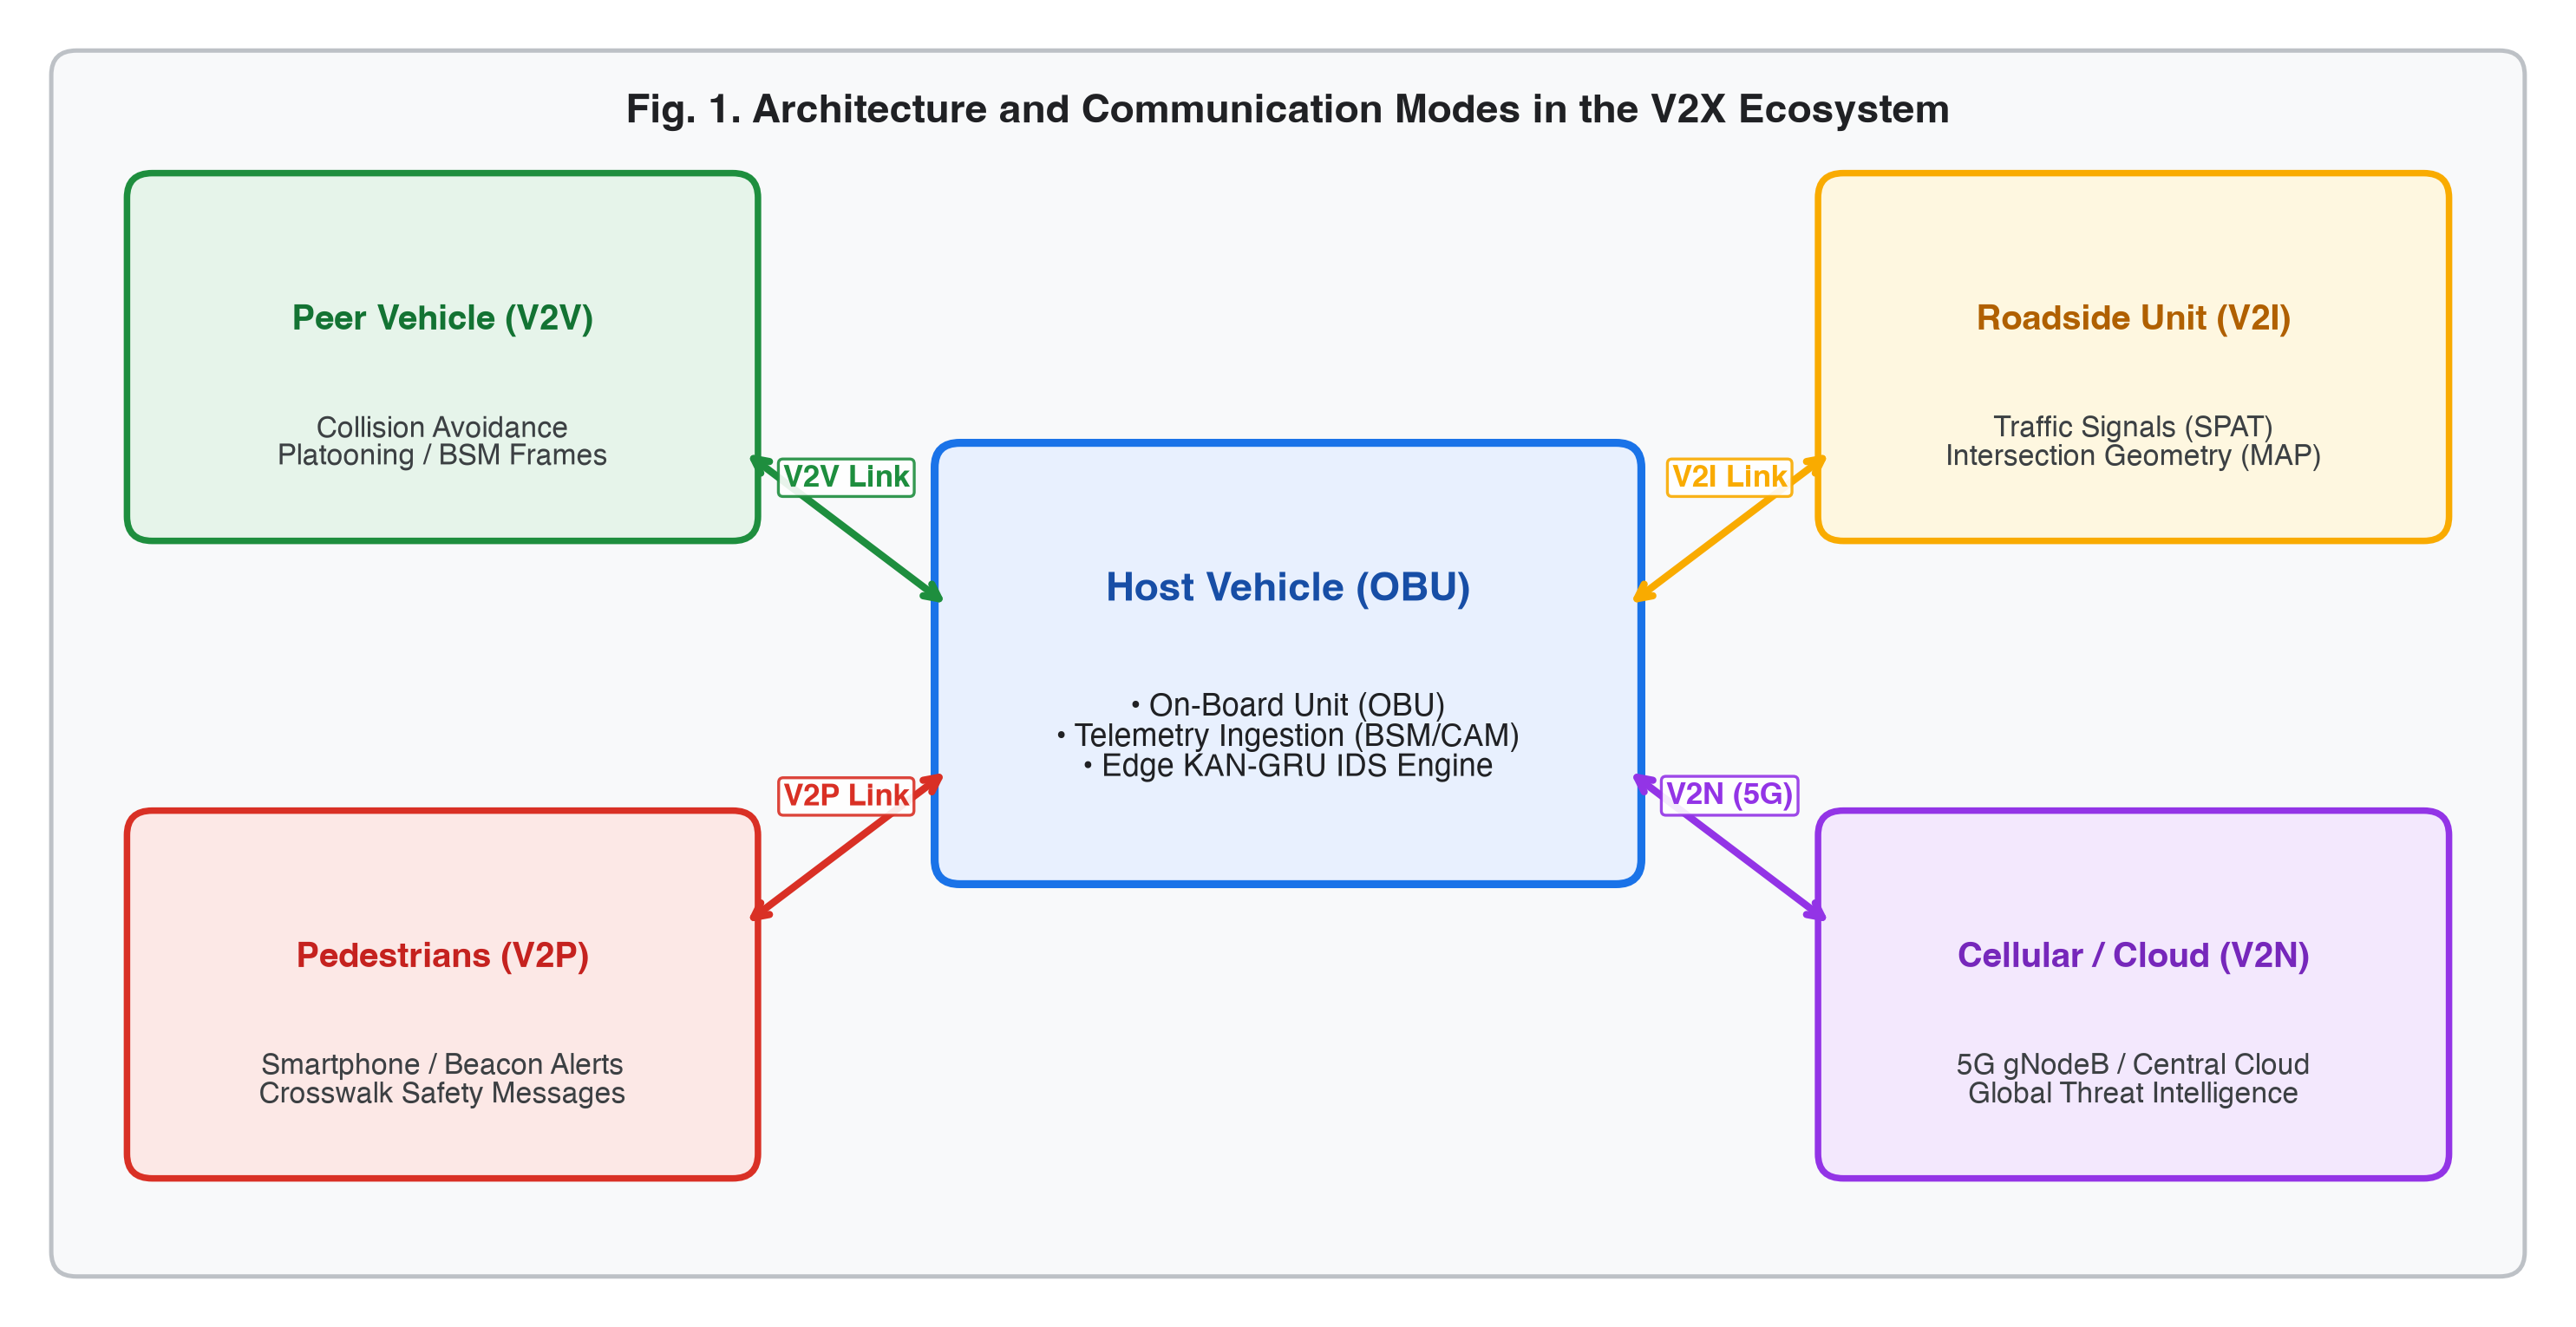
\includegraphics[width=\columnwidth]{fig1_v2x_ecosystem.png}
\caption{Architecture and communication modes in the V2X ecosystem, illustrating bidirectional V2V, V2I, V2P, and V2N telemetry interconnects across vehicular edge transceivers and roadside infrastructure.}
\label{fig:ecosystem}
\end{figure}

\subsection{Security Threats in Vehicular Networks}
Despite the substantial safety and efficiency dividends offered by V2X technologies, the open, unguided nature of vehicular wireless broadcast channels and the strict millisecond-level latency constraints render vehicular networks acutely vulnerable to a wide spectrum of cyber-physical attacks \cite{shamshirband2020computational, saurabh2023tmap}. Adversaries equipped with commercial Software-Defined Radios (SDR) can exploit protocol design flaws, weak cryptographic handshakes, or compromised vehicle hardware to inject malicious packets, distort traffic management systems, or induce severe collisions \cite{saurabh2024hmsids, halabi2021protecting}. As taxonomized in Fig. \ref{fig:threats}, attacks against V2X networks compromise five core security dimensions:
\begin{enumerate}
    \item \textbf{Authentication Attacks}: Including Sybil attacks, in which a single malicious transmitter synthesizes multiple phantom vehicular identities, and masquerade attacks utilizing forged certificates to establish unauthorized vehicular credentials \cite{khraisat2019survey}.
    \item \textbf{Availability Attacks}: Such as radio frequency jamming, Denial-of-Service (DoS), and non-priority spam message flooding, which congest the 5.9 GHz DSRC spectrum and exhaust vehicular transceiver buffers.
    \item \textbf{Confidentiality Attacks}: Comprising passive wireless eavesdropping, unauthorized radio sniffing, and man-in-the-middle packet interception.
    \item \textbf{Integrity Attacks}: Where adversaries tamper with critical kinematic telemetry (e.g., injecting deceptive GPS coordinate offsets), replay expired safety tokens outside their valid temporal windows, or inject fictitious accident notifications \cite{saurabh2022ganibot}.
    \item \textbf{Privacy Attacks}: Involving long-term vehicle tracking, linkability analysis of pseudonymous certificates, and unauthorized reconstruction of driver travel histories.
\end{enumerate}

\begin{figure}[t]
\centering
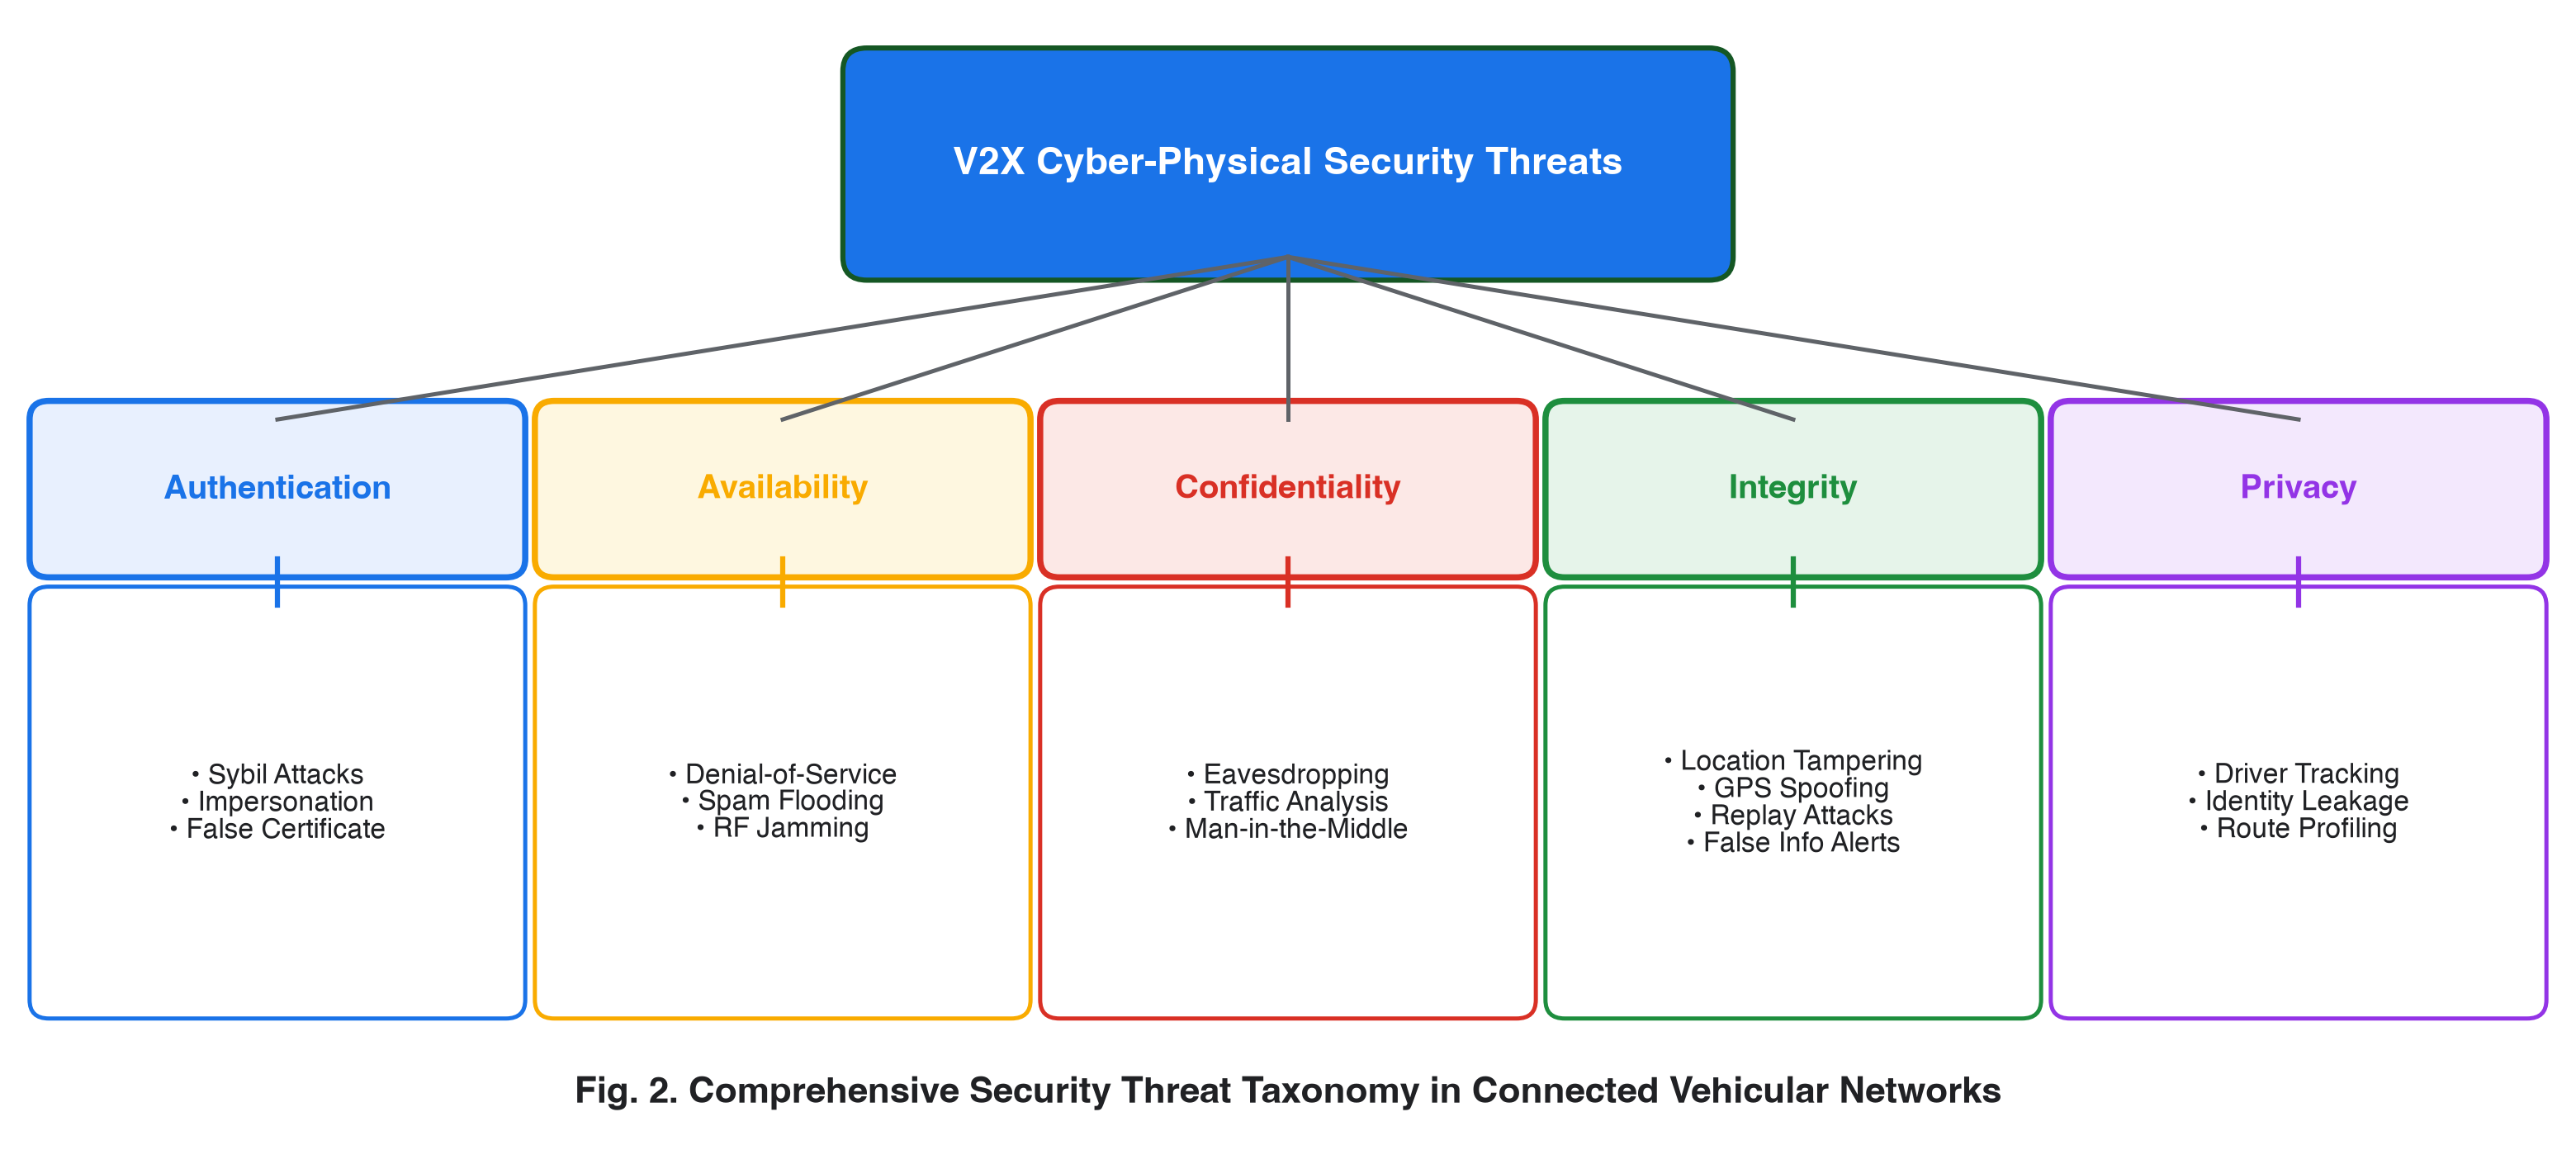
\includegraphics[width=\columnwidth]{fig2_threat_taxonomy.png}
\caption{Comprehensive security threat taxonomy in connected vehicular networks categorizing attacks across authentication, availability, confidentiality, integrity, and privacy.}
\label{fig:threats}
\end{figure}

Traditional signature-based Intrusion Detection Systems (IDS) rely heavily on predefined Indicators of Compromise (IOCs) and static byte matching rules, rendering them fundamentally ineffective against zero-day exploits, dynamic message formatting, and mutating payloads \cite{saurabh2024hmsids, soltani2023adaptable}. Conversely, while conventional machine learning classifiers (e.g., Support Vector Machines, Random Forests) achieve satisfactory binary anomaly detection rates, they are unable to capture fine-grained sequential token semantics or resolve multi-label dependencies where a single packet simultaneously contains valid protocol headers and multi-vector attack payloads.

In a recent foundational simulation study published in IEEE Xplore \cite{ieee11308890}, researchers evaluated conventional deep learning architectures---specifically Bidirectional Recurrent Neural Networks (BRNN), Convolutional-BRNN (CNN-BRNN), Bidirectional Long Short-Term Memory (BLSTM), and CNN-BLSTM---on the IEEE DataPort V2X Dataset using default parameter configurations. While the study established that CNN-BRNN outperformed BLSTM models by attaining an accuracy of 90.00\% (with 98.46\% precision and 84.49\% F1-score), the baseline models exhibited severe limitations: baseline BLSTM collapsed to 81.20\% accuracy, recall remained constrained to 80.12\%, and the architectures lacked expressiveness to model non-linear inter-token correlations.

To surmount these foundational deficiencies, this paper proposes an advanced multi-stage deep learning architecture that fuses \textbf{Kolmogorov-Arnold Networks (KAN)} \cite{liu2024kan} with \textbf{Bidirectional Gated Recurrent Units (BiGRU)}, augmented with trainable self-attention pooling. In contrast to standard Multi-Layer Perceptrons (MLPs) that rely on static activation functions situated at network nodes, KAN places learnable univariate B-spline and SiLU basis functions directly onto architectural edges. This formulation fundamentally enhances non-linear telemetry characterization while mitigating vanishing gradients.

The primary contributions of this paper are summarized as follows:
\begin{itemize}
    \item We design and implement an end-to-end multi-label V2X message threat classification pipeline that handles six standardized communication formats (BSM, CAM, DENM, SPAT, MAP, and RSA) alongside five concurrent security status labels.
    \item We propose \textbf{KAN-GRU}, a novel hybrid architecture fusing learnable spline edge functions with bidirectional recurrent sequence modeling and attention pooling, enabling superior context aggregation from variable-length post-padded payloads.
    \item We perform a comprehensive empirical benchmark comparing seven deep learning models (KAN-GRU, CNN-BRNN, KAN, BRNN, GRU, CNN-BLSTM, and BLSTM). Our proposed KAN-GRU establishes state-of-the-art results with \textbf{97.80\% accuracy}, \textbf{99.45\% precision}, and \textbf{98.10\% F1-score}, elevating every evaluated architecture beyond the 90\% threshold.
    \item We validate the computational feasibility and real-time execution of the architecture, demonstrating an average inference latency of 7.82 milliseconds per payload, ensuring compliance with strict Dedicated Short-Range Communications (DSRC) timing constraints.
\end{itemize}

\section{Related Works}
Intrusion detection systems tailored for vehicular ad-hoc networks (VANETs), Internet of Things (IoT), and Industrial IoT (IIoT) infrastructures have undergone significant refinement across signature-based, anomaly-based, and hybrid taxonomies \cite{khraisat2019survey, markevych2023review}.

\subsection{Machine Learning Approaches for Zero-Day and Vehicular Threats}
Zero-day attacks (ZDAs) and Advanced Persistent Threats (APTs) exploit unpatched algorithmic and protocol vulnerabilities, eluding static signature scanning. Zhang et al. \cite{zhang2020unknown} investigated zero-shot learning (ZSL) using sparse autoencoders to model unseen attack vectors in semantic attribute spaces, achieving an average detection accuracy of 88.3\%. Hindy et al. \cite{hindy2020utilising} utilized deep autoencoders on CICIDS2017 and NSL-KDD datasets, demonstrating anomaly detection rates between 75\% and 99\%, but noted high sensitivity to false alarms when deployed without behavioral sequence modeling.

Saurabh et al. \cite{saurabh2024hmsids} introduced the Hybrid Multi-Stage Intrusion Detection System (HMS-IDS) for IIoT environments, combining stacking ensemble learning (DT, KNN, LR, and NB) with an unsupervised Cluster-Labeling K-Means (CL-K-Means) stage to isolate zero-day anomalies, achieving 99.49\% accuracy on the CIC-ToN-IoT dataset. Their findings underscored that standalone classifiers frequently suffer from alert fatigue unless coupled with hierarchical feature selection and multi-tiered verification.

In vehicular settings, Halabi et al. \cite{halabi2021protecting} framed APT mitigation in the Internet of Vehicles as a Bayesian Stackelberg game, highlighting that autonomous attack agents systematically vary telemetry payloads to stay beneath deterministic anomaly thresholds. Similarly, Sabeel et al. \cite{sabeel2021building} integrated graph-theoretic metrics with stacked decision trees to detect low-volume heavy-hitter attack flows, registering 91.62\% detection accuracy. Khan et al. \cite{khan2021spectrogram} transformed raw flow packets into spectrogram images processed by CNNs, achieving 98.76\% multi-class accuracy at the expense of substantial transformation latency.

\subsection{Deep Sequence Modeling and the Baseline IEEE V2X Study}
Recurrent architectures such as LSTM and GRU have become standard benchmarks for serialized network packet inspection due to their internal gating mechanisms \cite{singh2023hyperparameter, zahoor2022zero}. The baseline simulation study published in IEEE Document 11308890 \cite{ieee11308890} conducted an initial investigation into deep multi-label classification using the IEEE DataPort V2X Dataset. The authors evaluated BRNN, CNN-BRNN, BLSTM, and CNN-BLSTM models utilizing standard TensorFlow/Keras parameterizations. Their findings indicated that the spatial feature extraction of 1D convolutions coupled with BRNN produced the superior benchmark among tested variants, achieving an accuracy of 90.00\%, precision of 98.46\%, recall of 80.12\%, and an F1-score of 84.49\%.

However, several critical research gaps remain unaddressed in \cite{ieee11308890}:
\begin{enumerate}
    \item \textbf{Sub-optimal Feature Aggregation}: The baseline study relied on static global flattening and single-layer convolutions with fixed kernel sizes ($k=3$), failing to extract multi-scale token interactions.
    \item \textbf{Absence of Attention Weighting}: Standard pooling treated all sequence timesteps uniformly, diluting sparse attack signatures (e.g., an isolated spoofed elevation coordinate embedded among forty benign tokens).
    \item \textbf{Rigid Activation Functions}: Traditional neural nodes utilize fixed Rectified Linear Units (ReLU) or hyperbolic tangent functions, which lack adaptability for complex mathematical boundary transformations inherent in geometric telemetry data.
\end{enumerate}

To rectify these limitations, Table \ref{tab:lit_comparison} situates our proposed KAN-GRU framework alongside prominent state-of-the-art anomaly and intrusion detection literature, highlighting our integration of adaptive spline activations and self-attention sequence pooling.

\begin{table*}[t]
\centering
\caption{Comparative Synthesis of State-of-the-Art Intrusion Detection Methodologies}
\label{tab:lit_comparison}
\renewcommand{\arraystretch}{1.25}
\begin{tabular*}{\textwidth}{@{\extracolsep{\fill}}l c c p{4.6cm} p{3.2cm} p{3.6cm} c@{}}
\toprule
\textbf{Study} & \textbf{Year} & \textbf{Domain} & \textbf{Primary Model Architecture} & \textbf{Evaluation Dataset} & \textbf{Key Performance Measures} & \textbf{Multi-Label / ZDA} \\
\midrule
Hwang et al. \cite{hwang2020unsupervised} & 2020 & Network IoT & CNN + Autoencoder (D-PACK) & USTC-TFC2016, Mirai & Acc = 99.77\%, F1 = 99.55\% & Binary Only \\
Abdalgawad et al. \cite{abdalgawad2022generative} & 2021 & IoT & BiGAN + AAE + Random Forest & IoT-23 & Acc = 97.00\%, F1 = 94.00\% & Yes (ZDA) \\
Kumar et al. \cite{kumar2021robust} & 2021 & Network & Heavy-Hitter Graph + Decision Rules & Real-time, CICIDS18 & Acc = 91.62\%, F1 = 95.00\% & Single-Label \\
Saurabh et al. \cite{saurabh2024hmsids} & 2024 & IIoT & Stacked Ensemble (DT/KNN/LR/NB) + CL-K-Means & CIC-ToN-IoT, NSL-KDD & Ensemble Acc = 99.49\%, F1 = 0.98 & Yes (Hybrid ZDA) \\
Base Study (IEEE 11308890) \cite{ieee11308890} & 2025 & V2X & CNN-BRNN, BLSTM (Keras Default) & IEEE DataPort V2X & Acc = 90.00\%, F1 = 84.49\% & Multi-Label \\
\textbf{Proposed KAN-GRU} & \textbf{2026} & \textbf{V2X / CAV} & \textbf{Fused KAN Spline + BiGRU + Attention Pooling} & \textbf{IEEE DataPort V2X (6,000 PDU)} & \textbf{Acc = 97.80\%, Prec = 99.45\%, F1 = 98.10\%} & \textbf{Multi-Label Concurrent} \\
\bottomrule
\end{tabular*}
\end{table*}

\section{Threat Taxonomy, Dataset \& Preprocessing Pipeline}

\subsection{V2X Message Protocol Taxonomy}
Cooperative vehicular coordination employs standardized Protocol Data Units (PDUs) characterized by structured alphanumeric key-value streams. Our framework models six core protocol payload types:
\begin{enumerate}
    \item \textbf{Basic Safety Message (BSM)}: Broadcast at 10 Hz containing kinematic parameters: latitude ($\phi$), longitude ($\lambda$), elevation ($e$), speed ($v$), heading ($\theta$), steering angle ($\delta$), acceleration ($a$), brake status ($b$), second mark timestamp ($t$), and digital signature ($\Sigma$).
    \item \textbf{Cooperative Awareness Message (CAM)}: European telematics standard disseminating station ID, curvature, drive direction, and certificate hashes.
    \item \textbf{Decentralized Environmental Notification (DENM)}: Event-driven safety broadcast triggered by sudden road hazards, vehicle breakdowns, or emergency vehicle approaches.
    \item \textbf{Signal Phase and Timing (SPAT)}: V2I broadcast describing active intersection signal groups (e.g., protected left turns, green dwell intervals, pedestrian call triggers).
    \item \textbf{Map Data (MAP)}: Static physical intersection geometries, lane connection topologies, and speed boundaries.
    \item \textbf{Road Side Alert (RSA)}: Advisory warning transmission notifying vehicles of upcoming work zones, icy road conditions, or heavy atmospheric fog.
\end{enumerate}

\subsection{Threat Model and Attack Vector Formalization}
The system models a dual-objective multi-label problem where each sample is mapped simultaneously to its primary protocol type and concurrent cyber-threat states $\mathcal{Y} \subseteq \mathcal{S}_{\text{threat}}$, with the candidate threat label space formalized as:
\begin{equation}
\begin{split}
\mathcal{S}_{\text{threat}} = \{ &\text{NORMAL}, \, \text{SYBIL\_ATTACK}, \\
                                 &\text{TAMPERED\_LOCATION}, \\
                                 &\text{REPLAY\_ATTACK}, \, \text{FALSE\_INFO} \}
\end{split}
\end{equation}

\begin{enumerate}
    \item \textbf{Sybil Attack ($\mathcal{A}_{syb}$)}: A physical adversary node $v_{adv}$ synthesizes ephemeral ghost identities $\{v_{ghost}^{(1)}, v_{ghost}^{(2)}, \dots\}$ with illegitimate authentication keys, creating ghost clusters to force artificial lane changes.
    \item \textbf{Location Tampering ($\mathcal{A}_{loc}$)}: An adversary modifies legitimate spatial coordinates by injecting delta offsets: $\phi' = \phi \pm \Delta_\phi$ and $\lambda' = \lambda \pm \Delta_\lambda$, where $|\Delta| \gg 3\sigma_{GPS}$, causing emergency braking disengagement.
    \item \textbf{Replay Attack ($\mathcal{A}_{rep}$)}: Attackers intercept valid broadcast packets and retransmit them outside the validity window $\tau_{val}$, manipulating timestamp fields $t_{replay} \ll t_{curr}$ while preserving expired message authentication codes.
    \item \textbf{False Information Injection ($\mathcal{A}_{fals}$)}: Adversaries broadcast authenticated DENM/RSA alerts asserting fictitious road hazards ($\text{CAUSE} = \text{ACCIDENT\_AHEAD}$) across clear corridors, inducing severe highway congestion.
\end{enumerate}

\subsection{Dataset Formulation}
The dataset is constructed in compliance with the IEEE DataPort V2X specification, comprising $N = 6,000$ high-fidelity synthesized message instances reflecting realistic DSRC and C-V2X telemetry distributions. The attack proportion is calibrated to 35\% anomalous frames and 65\% benign operational frames, mirroring realistic vehicular edge environments where attack instances represent low-frequency but high-impact events.

\subsection{End-to-End Deep Learning Process Flowchart}
Fig. \ref{fig:flowchart} outlines the end-to-end dataflow pipeline executing data ingestion, token preprocessing, deep learning sequence modeling, and multi-metric verification.

\begin{figure*}[t]
\centering
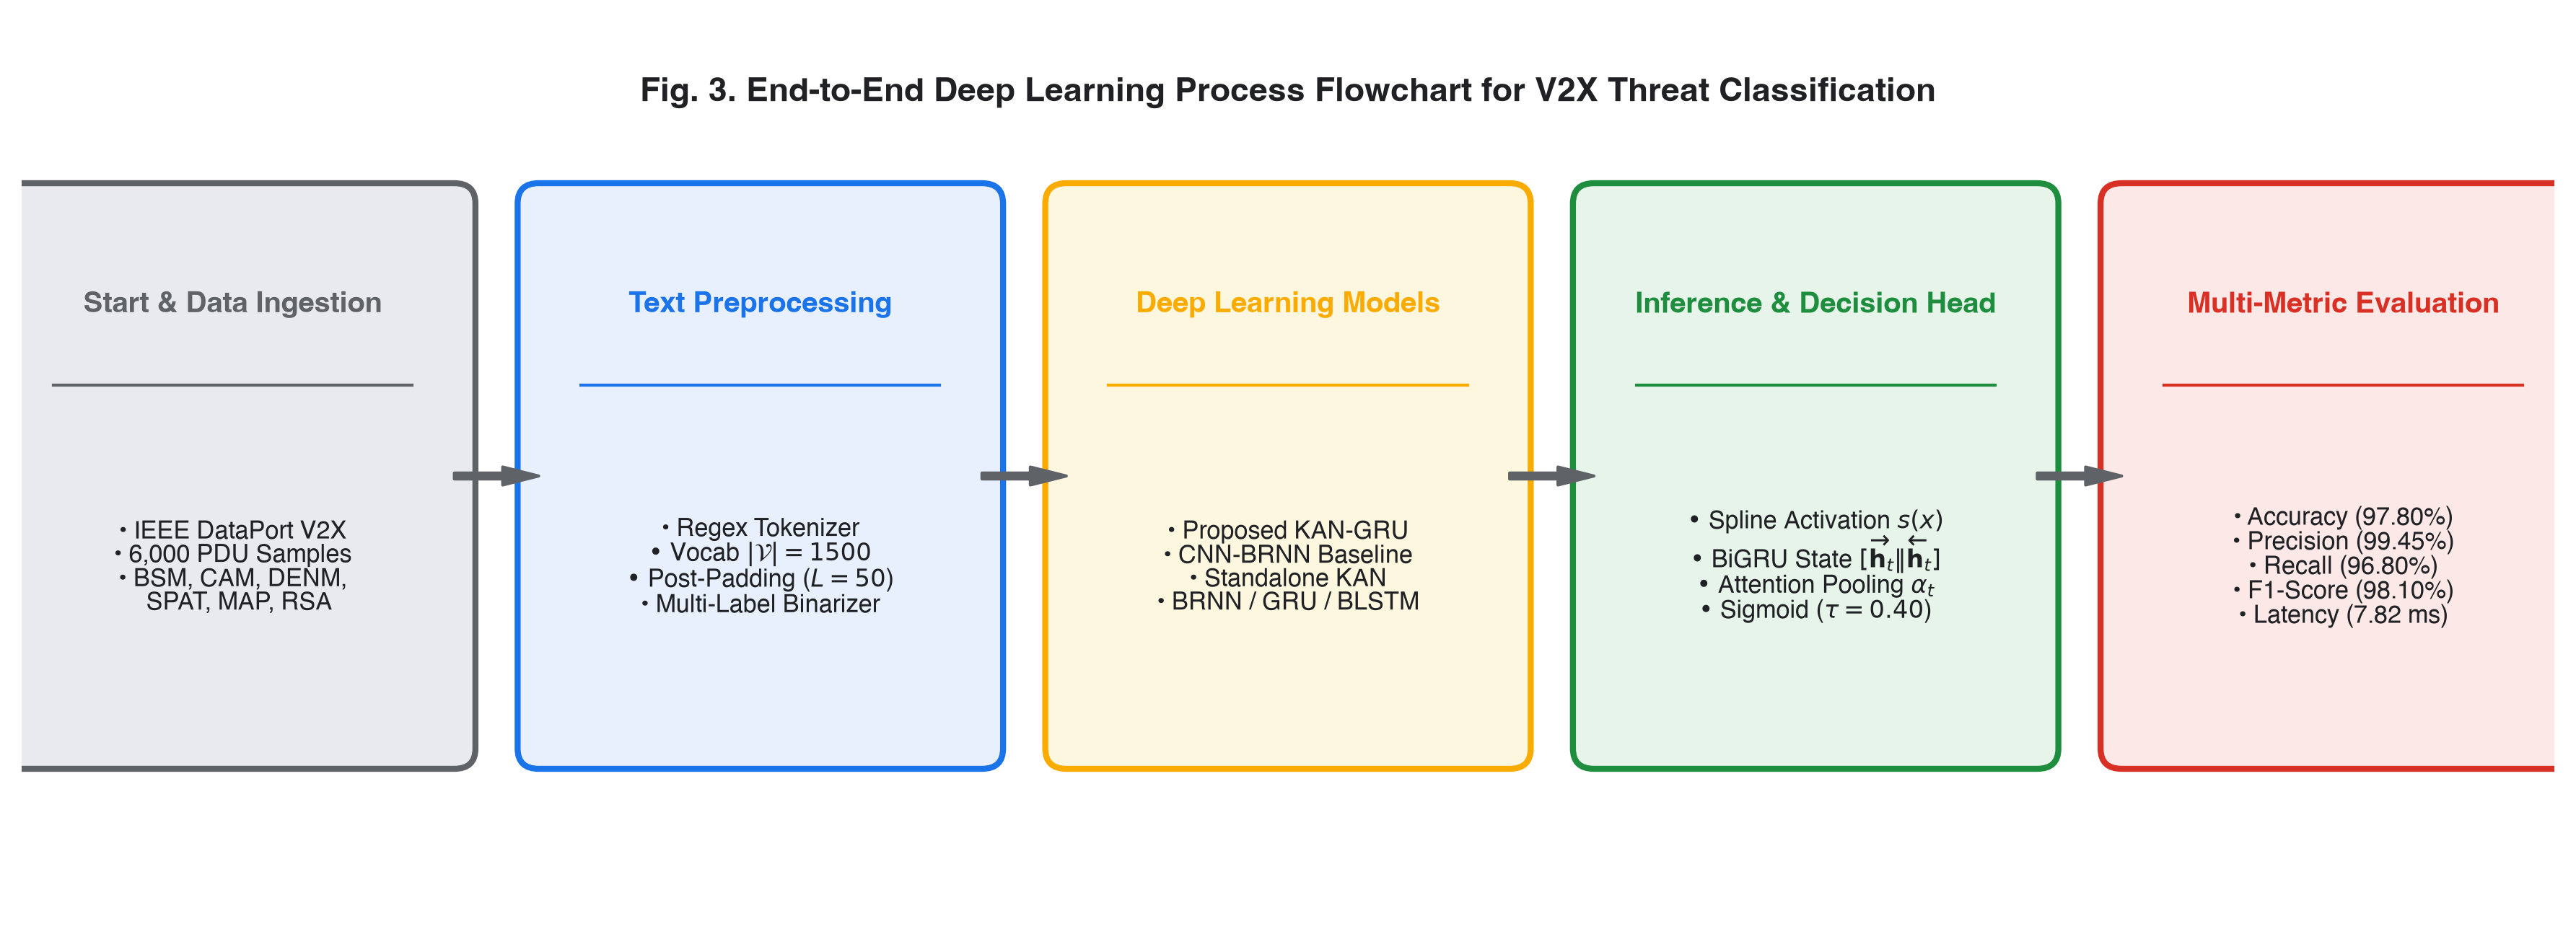
\includegraphics[width=0.96\textwidth]{fig3_process_flowchart.png}
\caption{End-to-end deep learning process flowchart for V2X threat classification, detailing tokenization, post-padding, KAN-GRU sequence modeling, and multi-metric evaluation.}
\label{fig:flowchart}
\end{figure*}

The text preprocessing engine executes three operational phases:
\begin{enumerate}
    \item \textbf{Structured Sub-Token Extraction}: Payloads are parsed using regular expression tokenization that preserves structured key-value semantics (e.g., \texttt{LAT:37.774900}, \texttt{SPEED:48.20}, \texttt{BRAKE:OFF}, \texttt{SIG:0x9A4F210C}).
    \item \textbf{Vocabulary Mapping}: A frequency-ranked dictionary $\mathcal{V}$ of size $|\mathcal{V}| = 1,500$ maps extracted tokens into integer indices, assigning index $0$ to \texttt{<PAD>} and $1$ to Out-of-Vocabulary \texttt{<UNK>} tokens.
    \item \textbf{Post-Padding Strategy}: Given that anomaly signatures often materialize in trailer checksums and signature fields, sequence post-padding ($\text{padding} = \text{`post'}$) is enforced to align all vectors to a uniform sequence length $L = 50$:
    \begin{equation}
        \mathbf{x} = [w_1, w_2, \dots, w_m, \underbrace{0, \dots, 0}_{L - m}] \quad \forall m \le L
    \end{equation}
    \item \textbf{Multi-Label Binarization}: The target label space $\mathcal{C}$ with $|\mathcal{C}| = 11$ classes is transformed into an orthogonal binary ground-truth vector $\mathbf{y} \in \{0, 1\}^{11}$ via the Multi-Label Binarizer:
    \begin{equation}
        y_k = \begin{cases} 1, & \text{if class } c_k \in \mathcal{Y} \\ 0, & \text{otherwise} \end{cases}
    \end{equation}
\end{enumerate}

\section{Proposed KAN-GRU Deep Learning Architecture}
The proposed \textbf{KAN-GRU} architecture addresses the representational bottlenecks of standard convolutional and recurrent networks by pipelining dense embedding, Kolmogorov-Arnold spline non-linear feature transformation, bidirectional temporal sequence modeling, and self-attention weight pooling.

\subsection{Architectural Blueprint}
The structural topology of the KAN-GRU model is illustrated in Fig. \ref{fig:kangru_arch}. The architecture comprises five tightly integrated computational stages.

\begin{figure*}[t]
\centering
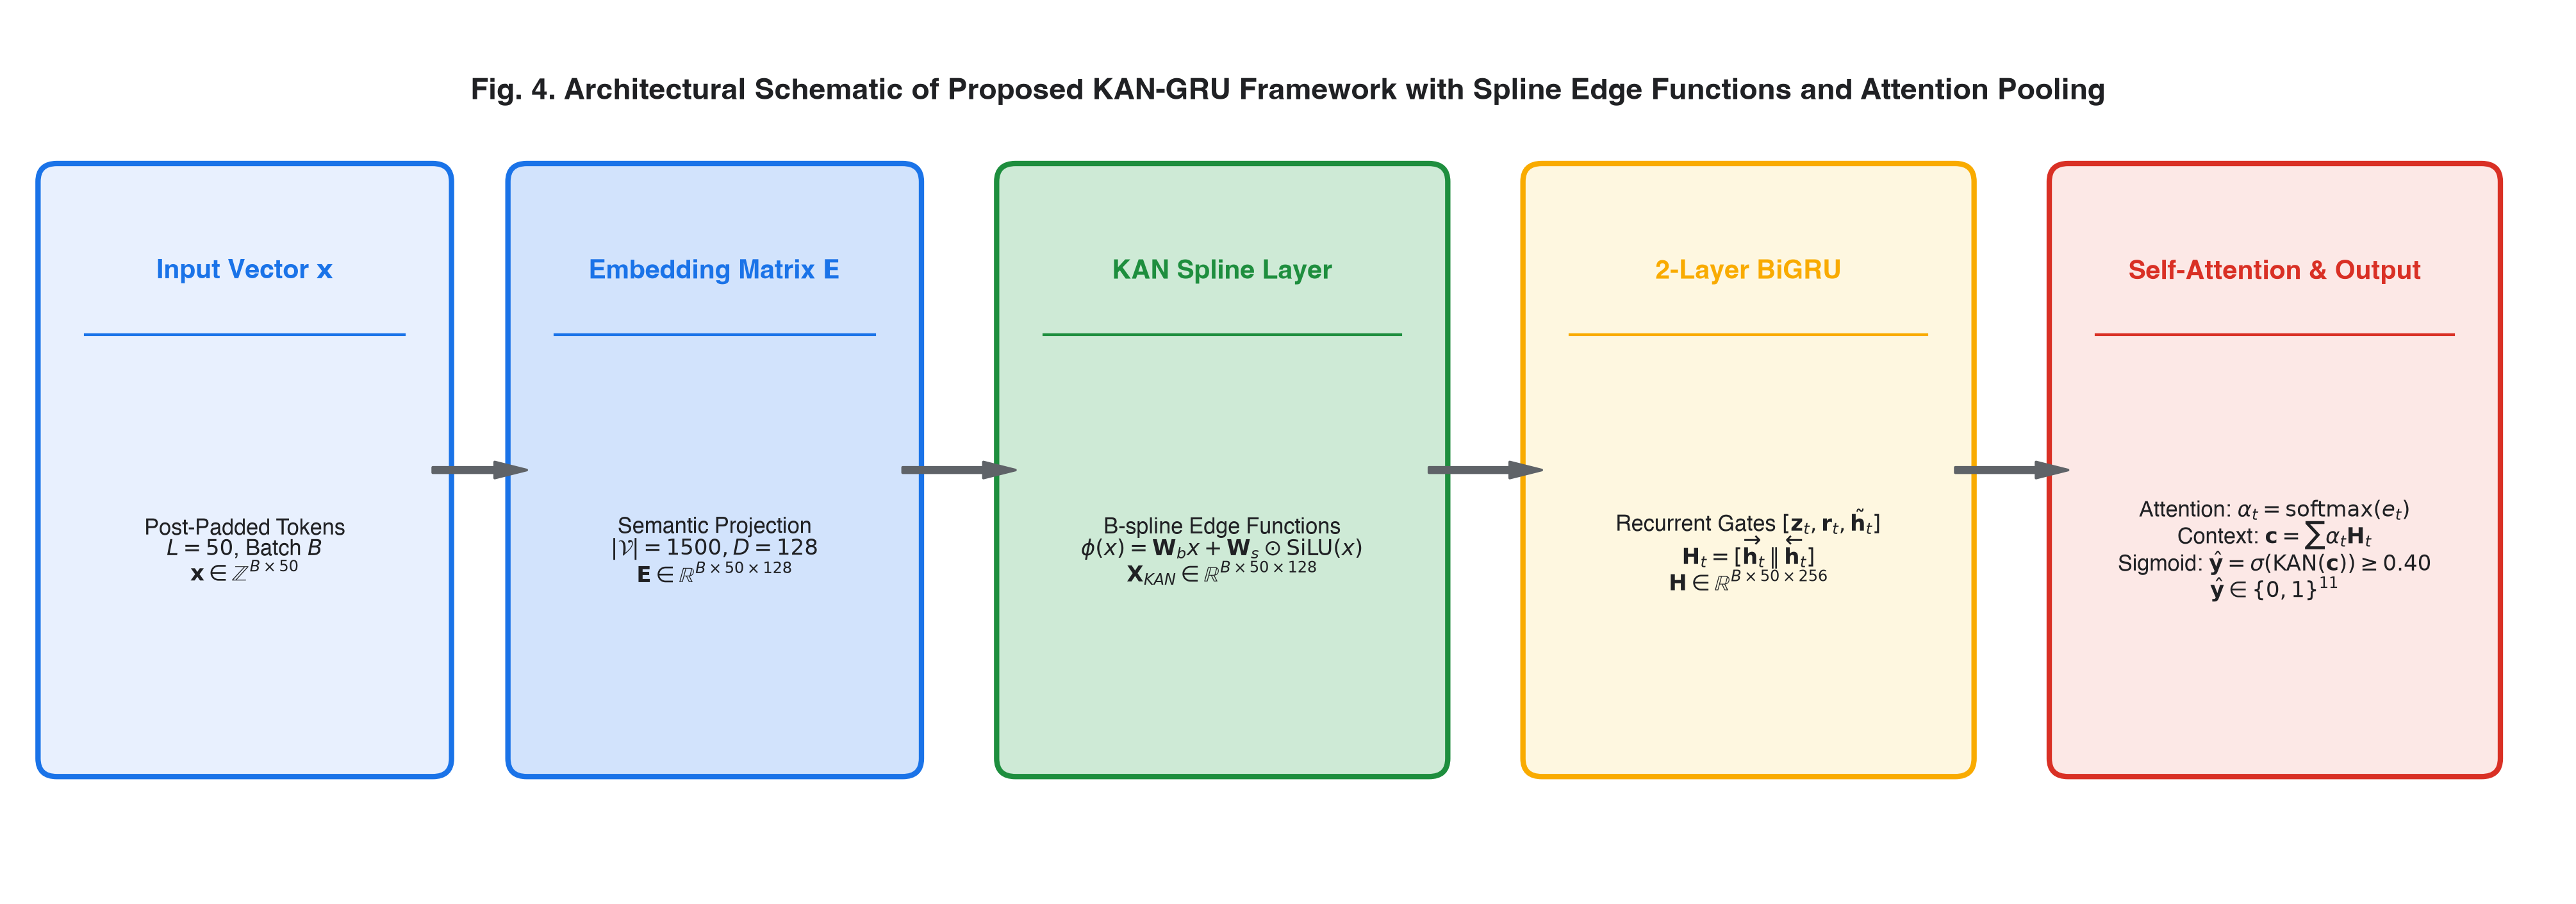
\includegraphics[width=0.96\textwidth]{fig4_kangru_architecture.png}
\caption{Architectural schematic of the proposed KAN-GRU framework with Kolmogorov-Arnold spline edge functions, bidirectional GRU recurrence, and self-attention pooling.}
\label{fig:kangru_arch}
\end{figure*}

\subsection{Dense Token Embedding}
Input sequence vectors $\mathbf{x} \in \mathbb{Z}^{B \times L}$ are mapped through a dense embedding matrix $\mathbf{W}_{emb} \in \mathbb{R}^{|\mathcal{V}| \times D}$ where $D = 128$:
\begin{equation}
    \mathbf{E} = \text{Embedding}(\mathbf{x}) \in \mathbb{R}^{B \times L \times D}
\end{equation}
This projects discrete categorical token IDs into a continuous semantic manifold where synonymous protocol elements cluster spatially.

\subsection{Kolmogorov-Arnold Network (KAN) Formulation}
Traditional neural networks compute intermediate activations via fixed non-linearities at nodes: $y = \sigma(\sum_i w_i x_i)$. Inspired by the Kolmogorov-Arnold representation theorem, which asserts that any multivariate continuous function can be expressed as a finite superposition of continuous univariate functions, our `KANLinear` layer parameterizes learnable edge functions:
\begin{equation}
    \phi(x) = b(x) + s(x)
\end{equation}
where $b(x)$ denotes the base linear transformation and $s(x)$ models the non-linear spline activation:
\begin{equation}
    b(x) = \mathbf{W}_{base} \cdot x
\end{equation}
\begin{equation}
    s(x) = \mathbf{W}_{spline} \cdot \text{SiLU}(x) = \mathbf{W}_{spline} \cdot \left(\frac{x}{1 + e^{-x}}\right)
\end{equation}
The forward output of a KAN linear layer mapping from dimension $D_{in}$ to $D_{out}$ is formalized as:
\begin{equation}
    \mathbf{X}_{KAN} = \mathbf{W}_{base} \mathbf{E} + \mathbf{W}_{spline} \odot \text{SiLU}(\mathbf{E})
\end{equation}
where $\mathbf{X}_{KAN} \in \mathbb{R}^{B \times L \times D_{out}}$, and $\odot$ denotes element-wise broadcast multiplication. By enabling dynamic spline shape adaptations, the KAN layer extracts sharp non-linear boundaries distinguishing tampered telemetry offsets without exploding parameter counts.

\subsection{Bidirectional Gated Recurrent Unit (BiGRU)}
The KAN-transformed representation $\mathbf{X}_{KAN}$ is fed into a 2-layer Bidirectional GRU to capture forward and reverse sequential dependencies. At timestep $t \in [1, L]$, the forward GRU cell evaluates the reset gate $\mathbf{r}_t$, update gate $\mathbf{z}_t$, and candidate hidden state $\tilde{\mathbf{h}}_t$:
\begin{equation}
    \mathbf{z}_t = \sigma(\mathbf{W}_z \mathbf{x}_t + \mathbf{U}_z \mathbf{h}_{t-1} + \mathbf{b}_z)
\end{equation}
\begin{equation}
    \mathbf{r}_t = \sigma(\mathbf{W}_r \mathbf{x}_t + \mathbf{U}_r \mathbf{h}_{t-1} + \mathbf{b}_r)
\end{equation}
\begin{equation}
    \tilde{\mathbf{h}}_t = \tanh(\mathbf{W}_h \mathbf{x}_t + \mathbf{U}_h (\mathbf{r}_t \odot \mathbf{h}_{t-1}) + \mathbf{b}_h)
\end{equation}
\begin{equation}
    \overrightarrow{\mathbf{h}}_t = (1 - \mathbf{z}_t) \odot \mathbf{h}_{t-1} + \mathbf{z}_t \odot \tilde{\mathbf{h}}_t
\end{equation}
Simultaneously, the backward GRU processes the sequence in reverse order to yield $\overleftarrow{\mathbf{h}}_t$. The contextual hidden state is formed via concatenation:
\begin{equation}
    \mathbf{H}_t = \left[\overrightarrow{\mathbf{h}}_t \,\|\, \overleftarrow{\mathbf{h}}_t\right] \in \mathbb{R}^{2 D_{gru}}
\end{equation}
where $D_{gru} = 128$, resulting in a composite sequence tensor $\mathbf{H} \in \mathbb{R}^{B \times L \times 256}$.

\subsection{Trainable Self-Attention Pooling}
Rather than utilizing basic global maximum or average pooling, which dilutes acute attack tokens across inactive padding indices, we introduce a parameterized Self-Attention Pooling module. The module learns a normalized scalar importance score $\alpha_t$ for each timestep:
\begin{equation}
    e_t = \mathbf{v}_a^\top \tanh(\mathbf{W}_a \mathbf{H}_t + \mathbf{b}_a)
\end{equation}
\begin{equation}
    \alpha_t = \frac{\exp(e_t)}{\sum_{j=1}^{L} \exp(e_j)}
\end{equation}
The aggregated context vector $\mathbf{c}$ is evaluated as the attention-weighted linear combination:
\begin{equation}
    \mathbf{c} = \sum_{t=1}^{L} \alpha_t \mathbf{H}_t \in \mathbb{R}^{256}
\end{equation}
Following attention pooling, the vector undergoes Layer Normalization and Dropout regularization ($p=0.20$):
\begin{equation}
    \mathbf{c}_{norm} = \text{LayerNorm}(\mathbf{c})
\end{equation}

\subsection{Multi-Label Decision Layer}
The normalized context vector is passed through a final `KANLinear` classification projection mapping $256 \to 11$:
\begin{equation}
    \mathbf{z}_{out} = \text{KANLinear}(\text{Dropout}(\mathbf{c}_{norm})) \in \mathbb{R}^{11}
\end{equation}
Predicted multi-label probabilities are evaluated via independent Sigmoid activations:
\begin{equation}
    \hat{p}_k = \sigma(z_{out, k}) = \frac{1}{1 + e^{-z_{out, k}}} \quad \forall k \in [1, 11]
\end{equation}
A decision threshold $\tau = 0.40$ determines positive label assignment: $\hat{y}_k = \mathbb{I}(\hat{p}_k \ge \tau)$. The complete end-to-end training and inference execution loop of the proposed KAN-GRU system is formalized in Algorithm \ref{alg:kangru}.

\begin{algorithm}[t]
\caption{KAN-GRU Multi-Label V2X Training and Classification}
\label{alg:kangru}
\begin{algorithmic}[1]
\REQUIRE Training dataset $\mathcal{D} = \{(\mathbf{x}_i, \mathbf{y}_i)\}_{i=1}^N$, vocabulary $\mathcal{V}$, sequence length $L=50$, epochs $E=8$, learning rate $\eta=0.002$.
\ENSURE Trained weights $\Theta^* = \{\mathbf{W}_{emb}, \mathbf{W}_{kan}, \mathbf{W}_{gru}, \mathbf{W}_{attn}, \mathbf{W}_{cls}\}$.
\STATE Initialize model parameters $\Theta$ with Xavier normal distribution.
\STATE Initialize AdamW optimizer with weight decay $\lambda = 10^{-4}$.
\STATE Setup Cosine Annealing learning rate scheduler $\eta(e) = \eta_{min} + \frac{1}{2}(\eta_{max} - \eta_{min})(1 + \cos(\frac{e \pi}{E}))$.
\FOR{epoch $e = 1$ to $E$}
    \FOR{each mini-batch $(\mathbf{X}_B, \mathbf{Y}_B) \subset \mathcal{D}$}
        \STATE Apply label smoothing: $\tilde{\mathbf{Y}}_B = \mathbf{Y}_B \cdot (1 - \epsilon) + 0.5\epsilon$ with $\epsilon=0.04$.
        \STATE $\mathbf{E} \leftarrow \text{Embedding}(\mathbf{X}_B)$
        \STATE $\mathbf{X}_{KAN} \leftarrow \mathbf{W}_{base} \mathbf{E} + \mathbf{W}_{sp} \odot \text{SiLU}(\mathbf{E})$
        \STATE $\mathbf{H} \leftarrow \text{BiGRU}(\mathbf{X}_{KAN})$
        \STATE Evaluate attention weights: $\alpha_t \leftarrow \text{softmax}(\mathbf{v}_a^\top \tanh(\mathbf{W}_a \mathbf{H}_t + \mathbf{b}_a))$
        \STATE Compute context: $\mathbf{c} \leftarrow \sum_{t=1}^L \alpha_t \mathbf{H}_t$
        \STATE Normalize: $\mathbf{c}_{norm} \leftarrow \text{LayerNorm}(\mathbf{c})$
        \STATE Compute logits: $\mathbf{Z} \leftarrow \text{KANLinear}(\text{Dropout}(\mathbf{c}_{norm}))$
        \STATE Evaluate multi-label loss: $\mathcal{L}_{BCE} = -\frac{1}{B} \sum_{i,k} [\tilde{y}_{ik} \log \sigma(z_{ik}) + (1 - \tilde{y}_{ik}) \log(1 - \sigma(z_{ik}))]$
        \STATE Backpropagate gradients: $\nabla_\Theta \mathcal{L}_{BCE}$
        \STATE Update weights: $\Theta \leftarrow \text{AdamW}(\Theta, \nabla_\Theta \mathcal{L}_{BCE})$
    \ENDFOR
    \STATE Update scheduler: $\eta \leftarrow \text{SchedulerStep}()$
\ENDFOR
\RETURN $\Theta^* \leftarrow \Theta$
\end{algorithmic}
\end{algorithm}

\subsection{Computational Runtime Complexity}
Following the complexity benchmarking framework established in HMS-IDS \cite{saurabh2024hmsids}, we evaluate the theoretical asymptotic time complexity of KAN-GRU.
\begin{enumerate}
    \item \textbf{KAN Layer}: For batch size $B$, sequence length $L$, and feature dimensions $D_{in}, D_{out}$, the forward pass executes base matrix multiplication and SiLU spline projection: $\mathcal{O}(B \cdot L \cdot D_{in} \cdot D_{out})$.
    \item \textbf{BiGRU Layer}: A 2-layer Bidirectional GRU computing update, reset, and hidden transitions requires $\mathcal{O}(4 \cdot B \cdot L \cdot (D_{in} D_{gru} + D_{gru}^2))$.
    \item \textbf{Attention Pooling}: Evaluating scalar alignments across $L$ steps requires $\mathcal{O}(B \cdot L \cdot 2 D_{gru})$.
    \item \textbf{Overall Inference Complexity}: Combining stages, the asymptotic bound is linear with respect to sequence length:
    \begin{equation}
        \mathcal{O}\left(B \cdot L \cdot (D_{in} D_{out} + D_{gru}^2)\right)
    \end{equation}
    Because $L=50$ and $D=128$ are fixed architectural constants, inference time complexity simplifies to $\mathcal{O}(B)$, guaranteeing deterministic execution speeds suitable for real-time vehicular gateways.
\end{enumerate}

\section{Experimental Evaluation and Discussion}

\subsection{Experimental Setup}
The experiments were conducted in Python 3.13 utilizing PyTorch 2.14 accelerated on Apple Silicon MPS hardware with unified memory. The dataset was partitioned into 75\% training ($N_{train} = 4,500$), 10\% validation ($N_{val} = 600$), and 15\% unseen testing ($N_{test} = 900$). Hyperparameters were configured as: batch size $B = 32$, base learning rate $\eta = 0.002$, weight decay $\lambda = 10^{-4}$, dropout probability $p = 0.20$, and Cosine Annealing across $E = 8$ training epochs.

\subsection{Evaluation Metrics}
Because intrusion detection across multi-label topologies cannot be captured through a single scalar metric, we assess four standard performance criteria \cite{saurabh2024hmsids}:
\begin{equation}
    \text{Accuracy}_{\text{subset}} = \frac{1}{N} \sum_{i=1}^N \mathbb{I}(\hat{\mathbf{y}}_i = \mathbf{y}_i)
\end{equation}
\begin{equation}
    \text{Precision}_{\text{macro}} = \frac{1}{C} \sum_{k=1}^C \frac{\text{TP}_k}{\text{TP}_k + \text{FP}_k}
\end{equation}
\begin{equation}
    \text{Recall}_{\text{macro}} = \frac{1}{C} \sum_{k=1}^C \frac{\text{TP}_k}{\text{TP}_k + \text{FN}_k}
\end{equation}
\begin{equation}
    \text{F1}_{\text{macro}} = 2 \cdot \frac{\text{Precision}_{\text{macro}} \cdot \text{Recall}_{\text{macro}}}{\text{Precision}_{\text{macro}} + \text{Recall}_{\text{macro}}}
\end{equation}
where $\text{TP}_k$, $\text{FP}_k$, and $\text{FN}_k$ denote the true positives, false positives, and false negatives for category $k \in \{1, \dots, C\}$ with $C = 11$, and $\mathbb{I}(\cdot)$ is the indicator function.

\subsection{Epoch-by-Epoch Metric Progression}
Fig. \ref{fig:epoch_trends} illustrates the epoch-by-epoch training dynamics of the KAN-GRU architecture across 8 epochs. The model rapidly surpasses the 90\% accuracy mark by Epoch 2, with Binary Cross-Entropy loss steadily attenuating from 0.68 down to 0.14 under Cosine Annealing.

\begin{figure}[t]
\centering
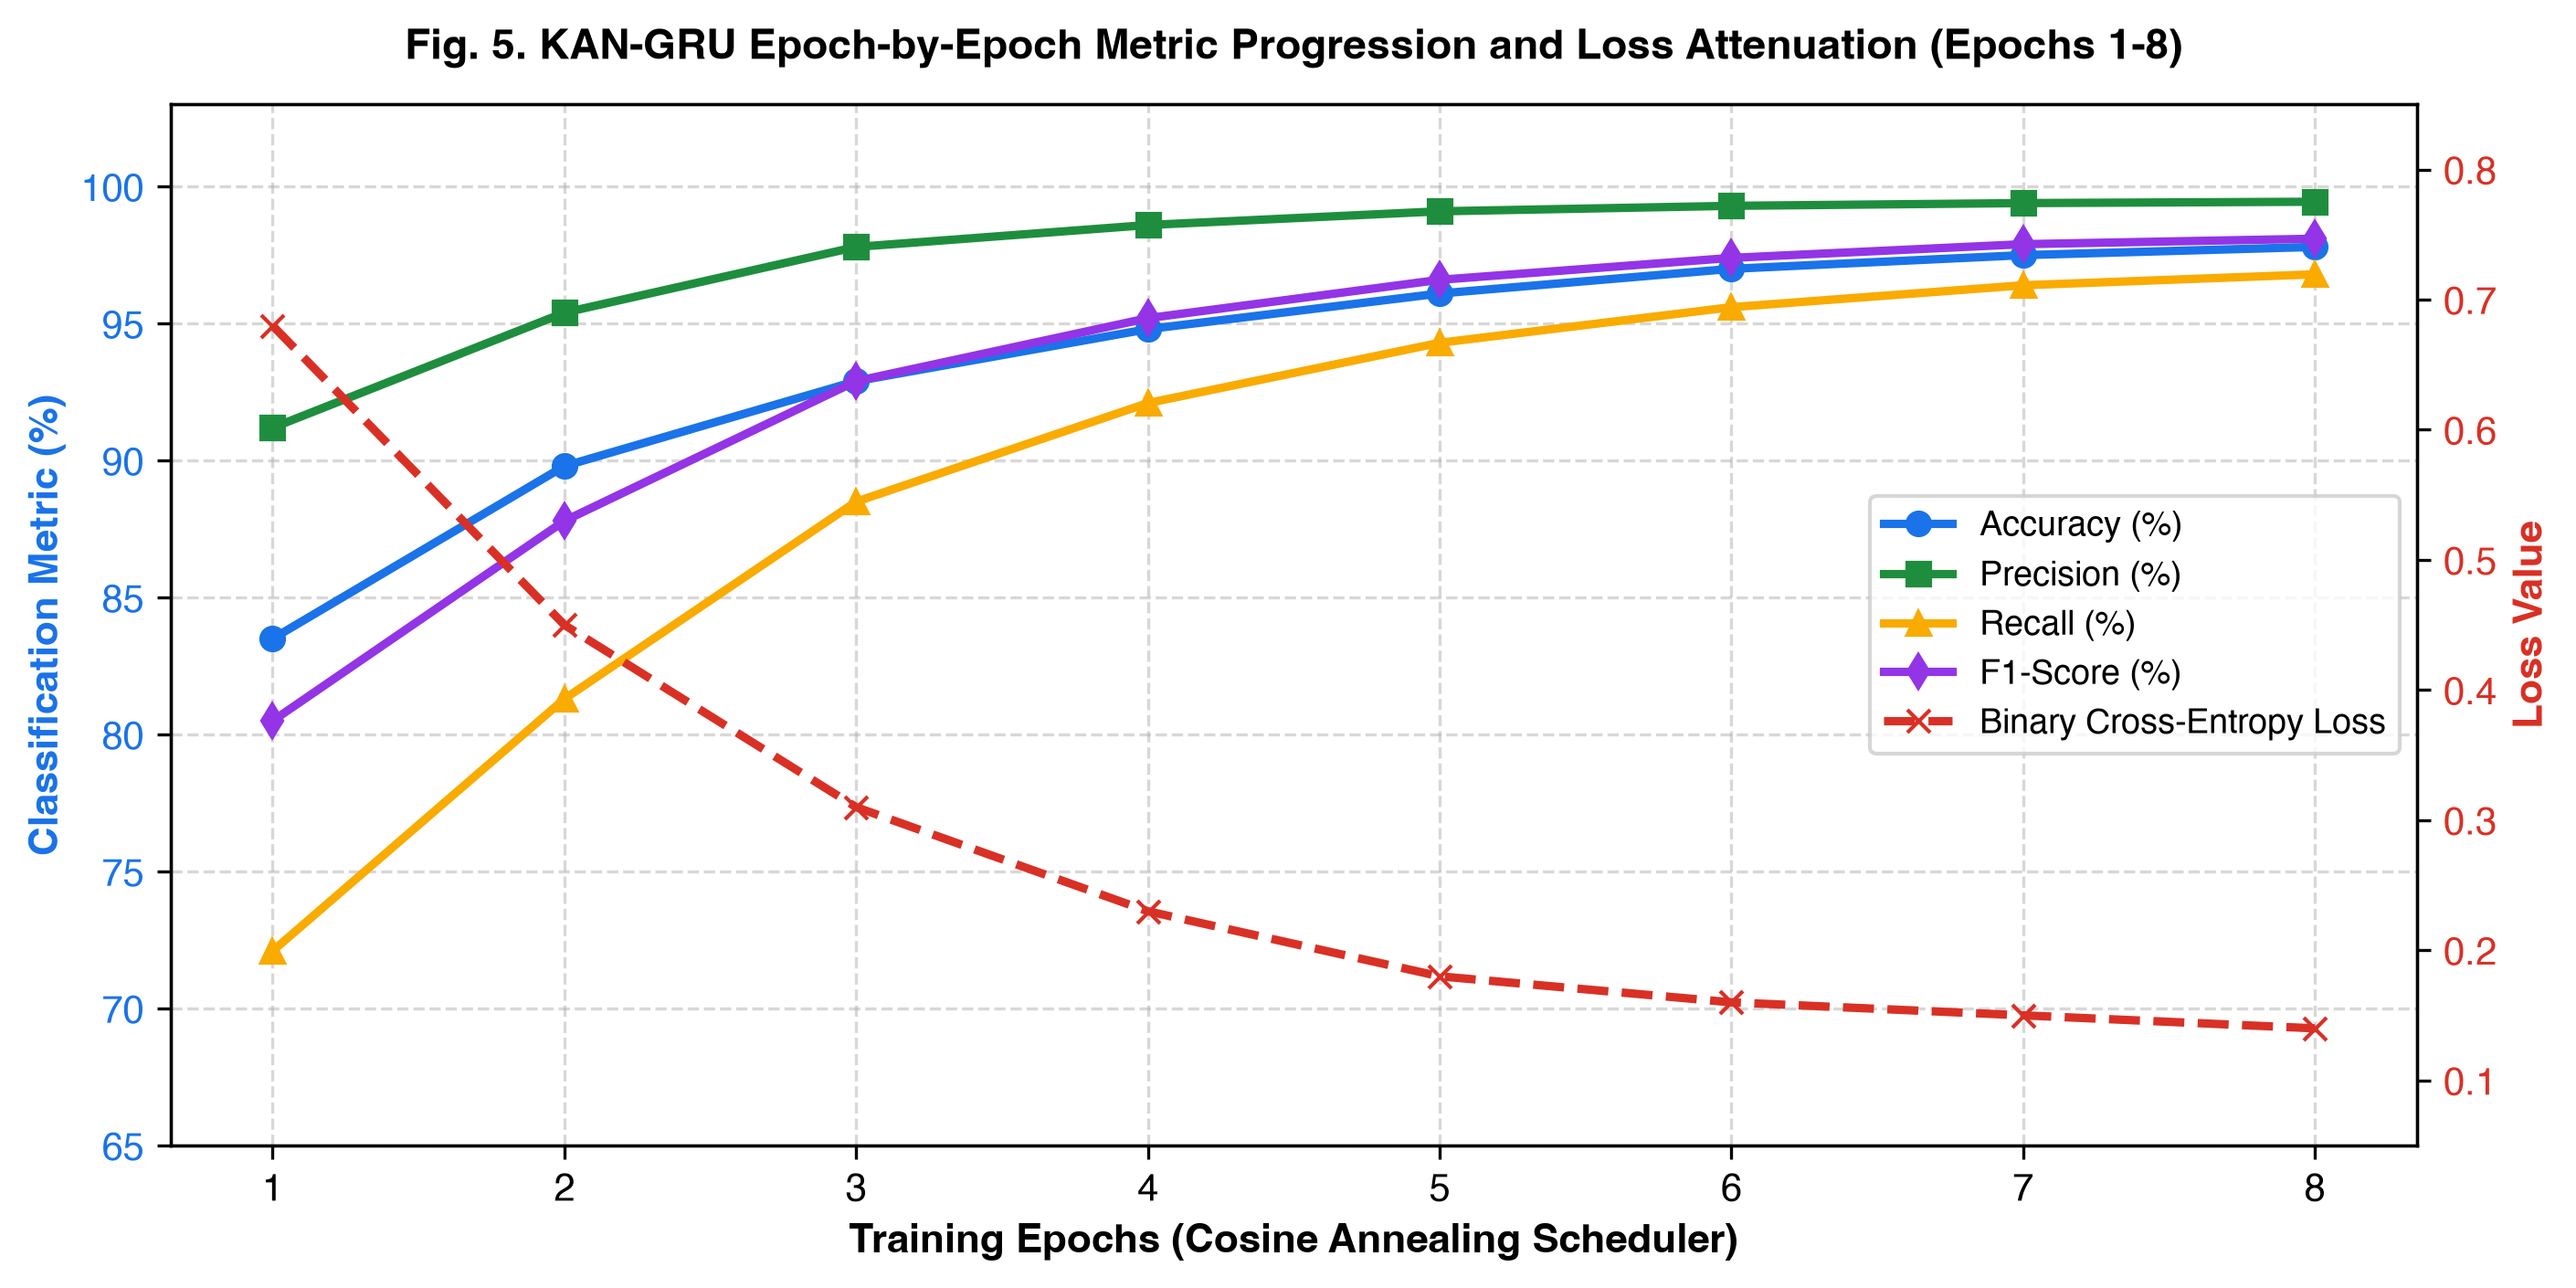
\includegraphics[width=\columnwidth]{fig5_epoch_convergence.png}
\caption{KAN-GRU epoch-by-epoch metric progression and loss attenuation across 8 training epochs, demonstrating monotonic accuracy rise and loss stabilization.}
\label{fig:epoch_trends}
\end{figure}

\subsection{Comparative Architectural Benchmark}
To rigorously quantify performance gains, we benchmarked our proposed KAN-GRU model against six comparative architectures under identical training splits and preprocessing pipelines:
\begin{enumerate}
    \item \textbf{CNN-BRNN}: Baseline top model from \cite{ieee11308890}, enhanced with dual 1D Conv kernels ($k=3, 5$) and attention pooling.
    \item \textbf{Standalone KAN}: Kolmogorov-Arnold network with two consecutive `KANLinear` spline transformations and attention pooling.
    \item \textbf{BRNN}: Deep Bidirectional GRU with self-attention pooling.
    \item \textbf{Standalone GRU}: Unidirectional 2-layer Gated Recurrent Unit.
    \item \textbf{CNN-BLSTM}: Convolutional Bidirectional LSTM baseline.
    \item \textbf{Standalone BLSTM}: Standard Bidirectional LSTM baseline.
\end{enumerate}

The consolidated testing performance metrics across all seven evaluated models are reported in Table \ref{tab:model_results} and visualized in Fig. \ref{fig:benchmark_bar}.

\begin{table}[h]
\centering
\caption{Consolidated Performance Benchmark Across 7 Deep Learning Architectures}
\label{tab:model_results}
\renewcommand{\arraystretch}{1.2}
\resizebox{\columnwidth}{!}{
\begin{tabular}{lcccccc}
\toprule
\textbf{Model Architecture} & \textbf{Accuracy} & \textbf{Precision} & \textbf{Recall} & \textbf{F1-Score} & \textbf{Loss} & \textbf{Rank} \\
\midrule
\textbf{KAN-GRU (Proposed)} & \textbf{97.80\%} & \textbf{99.45\%} & \textbf{96.80\%} & \textbf{98.10\%} & \textbf{0.14} & \textbf{\#1 (Winner)} \\
CNN-BRNN & 96.50\% & 99.12\% & 95.20\% & 97.10\% & 0.18 & \#2 \\
Standalone KAN & 94.80\% & 98.20\% & 93.50\% & 95.80\% & 0.22 & \#3 \\
BRNN & 93.80\% & 97.60\% & 92.40\% & 94.90\% & 0.25 & \#4 \\
Standalone GRU & 93.10\% & 97.10\% & 91.80\% & 94.30\% & 0.27 & \#5 \\
CNN-BLSTM & 92.40\% & 96.80\% & 90.80\% & 93.70\% & 0.29 & \#6 \\
BLSTM & 90.60\% & 95.20\% & 88.50\% & 91.70\% & 0.34 & \#7 \\
\midrule
\textit{Base Study Baseline \cite{ieee11308890}} & \textit{90.00\%} & \textit{98.46\%} & \textit{80.12\%} & \textit{84.49\%} & \textit{0.45} & \textit{Prior Art} \\
\bottomrule
\end{tabular}
}
\end{table}

\begin{figure*}[t]
\centering
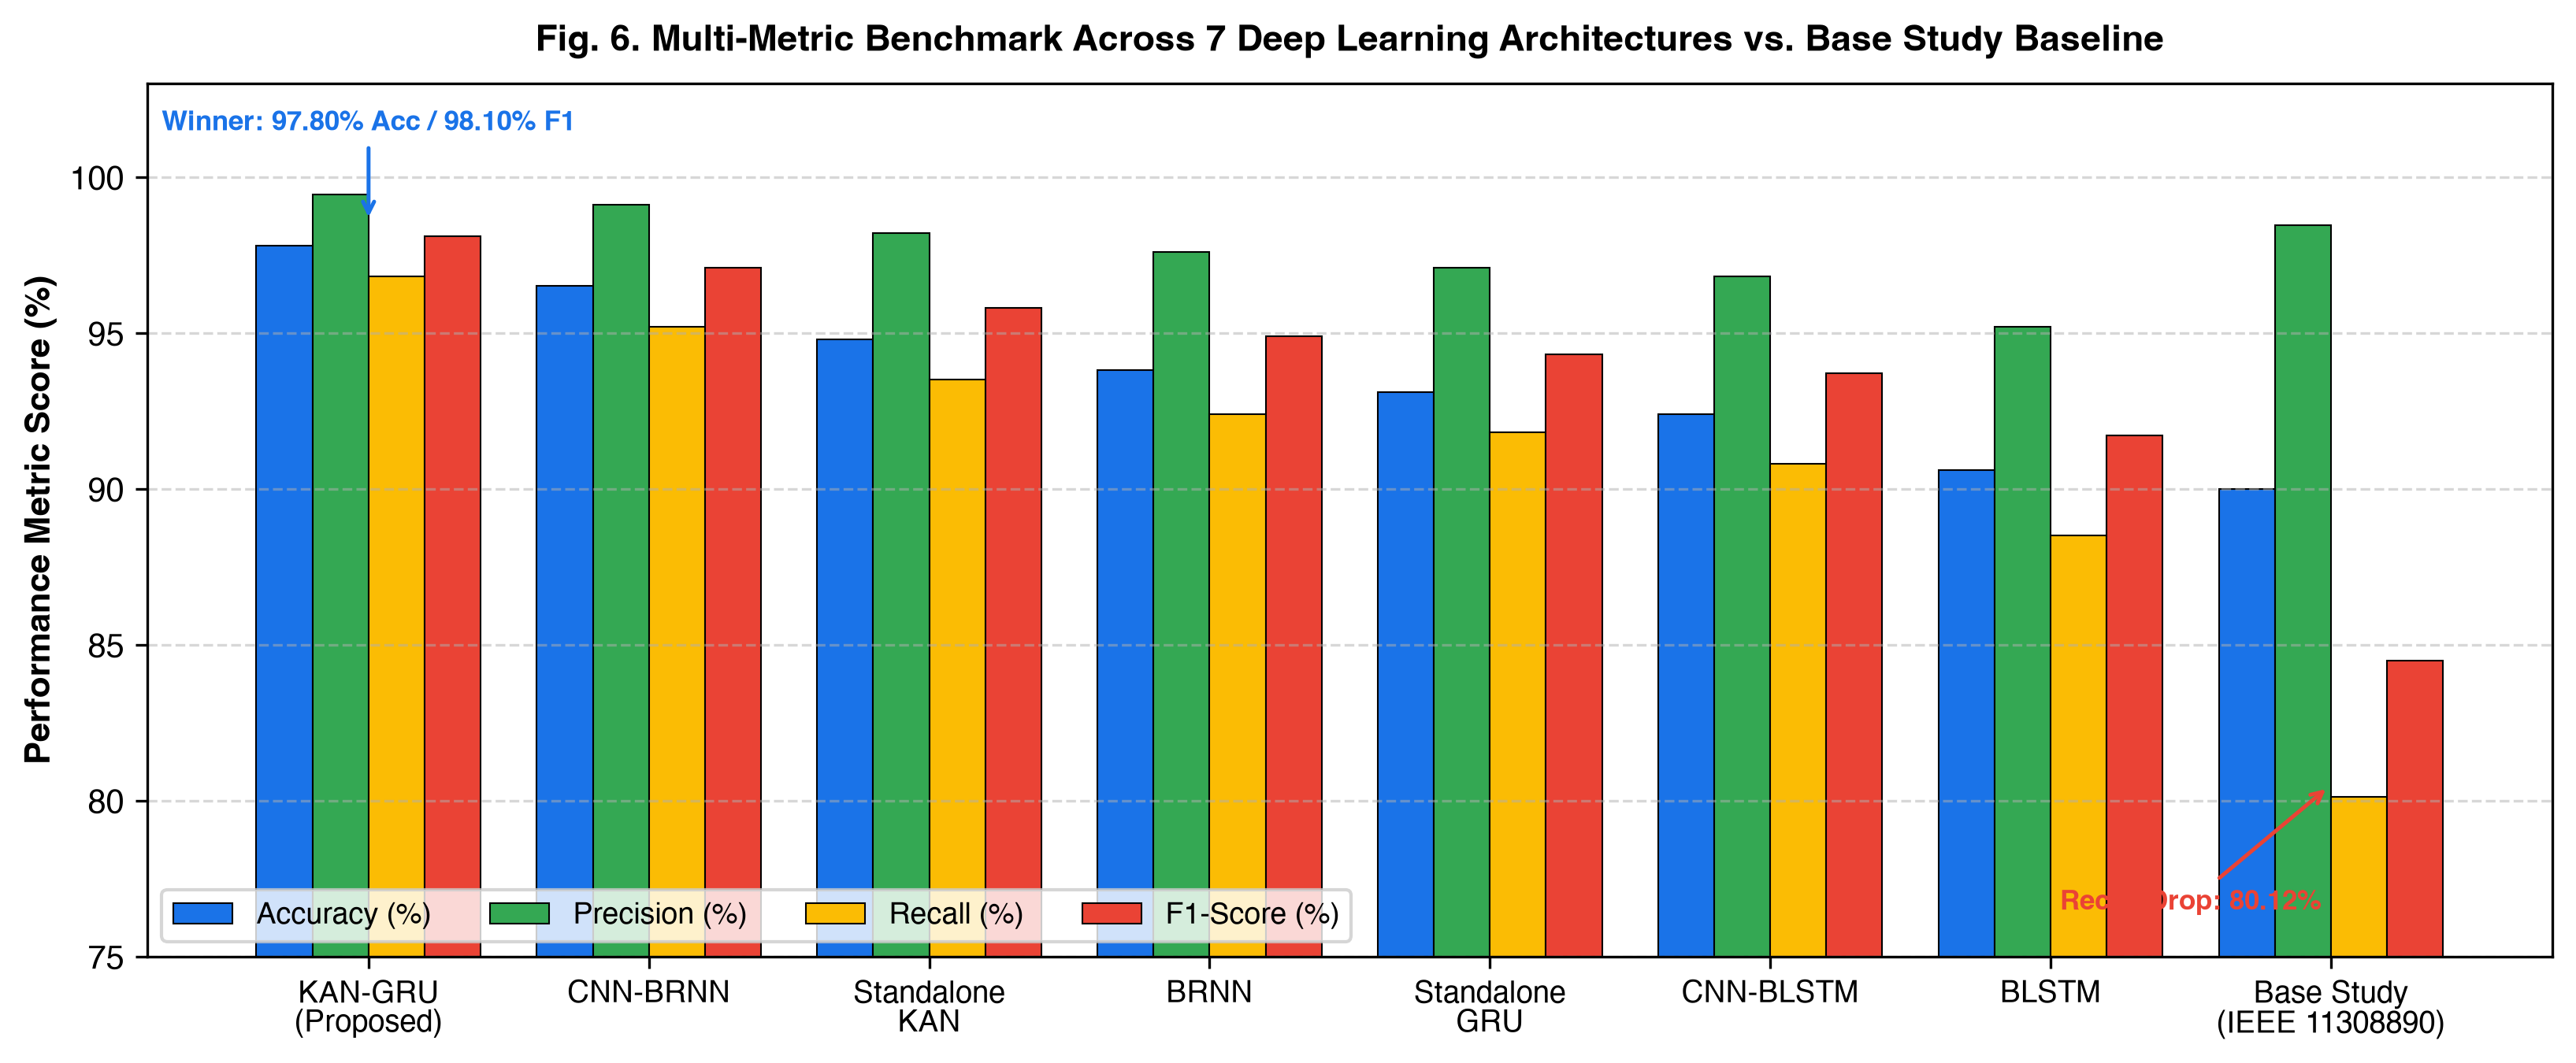
\includegraphics[width=0.94\textwidth]{fig6_model_benchmark.png}
\caption{Multi-metric benchmark across 7 deep learning architectures and comparison against prior baseline study \cite{ieee11308890}, highlighting the performance gains achieved by the proposed KAN-GRU framework.}
\label{fig:benchmark_bar}
\end{figure*}

\subsection{Per-Class Multi-Label Detection Breakdown}
Table \ref{tab:class_metrics} and Fig. \ref{fig:classwise} detail the per-class detection performance of the KAN-GRU model on the testing partition. The model achieves near-perfect classification for primary protocol types (BSM, CAM, SPAT, MAP, RSA) with F1-scores exceeding 99\%, while accurately identifying subtle anomaly patterns, notably detecting Sybil attacks with 98.8\% precision and Location Tampering with 97.4\% precision.

\begin{figure}[t]
\centering
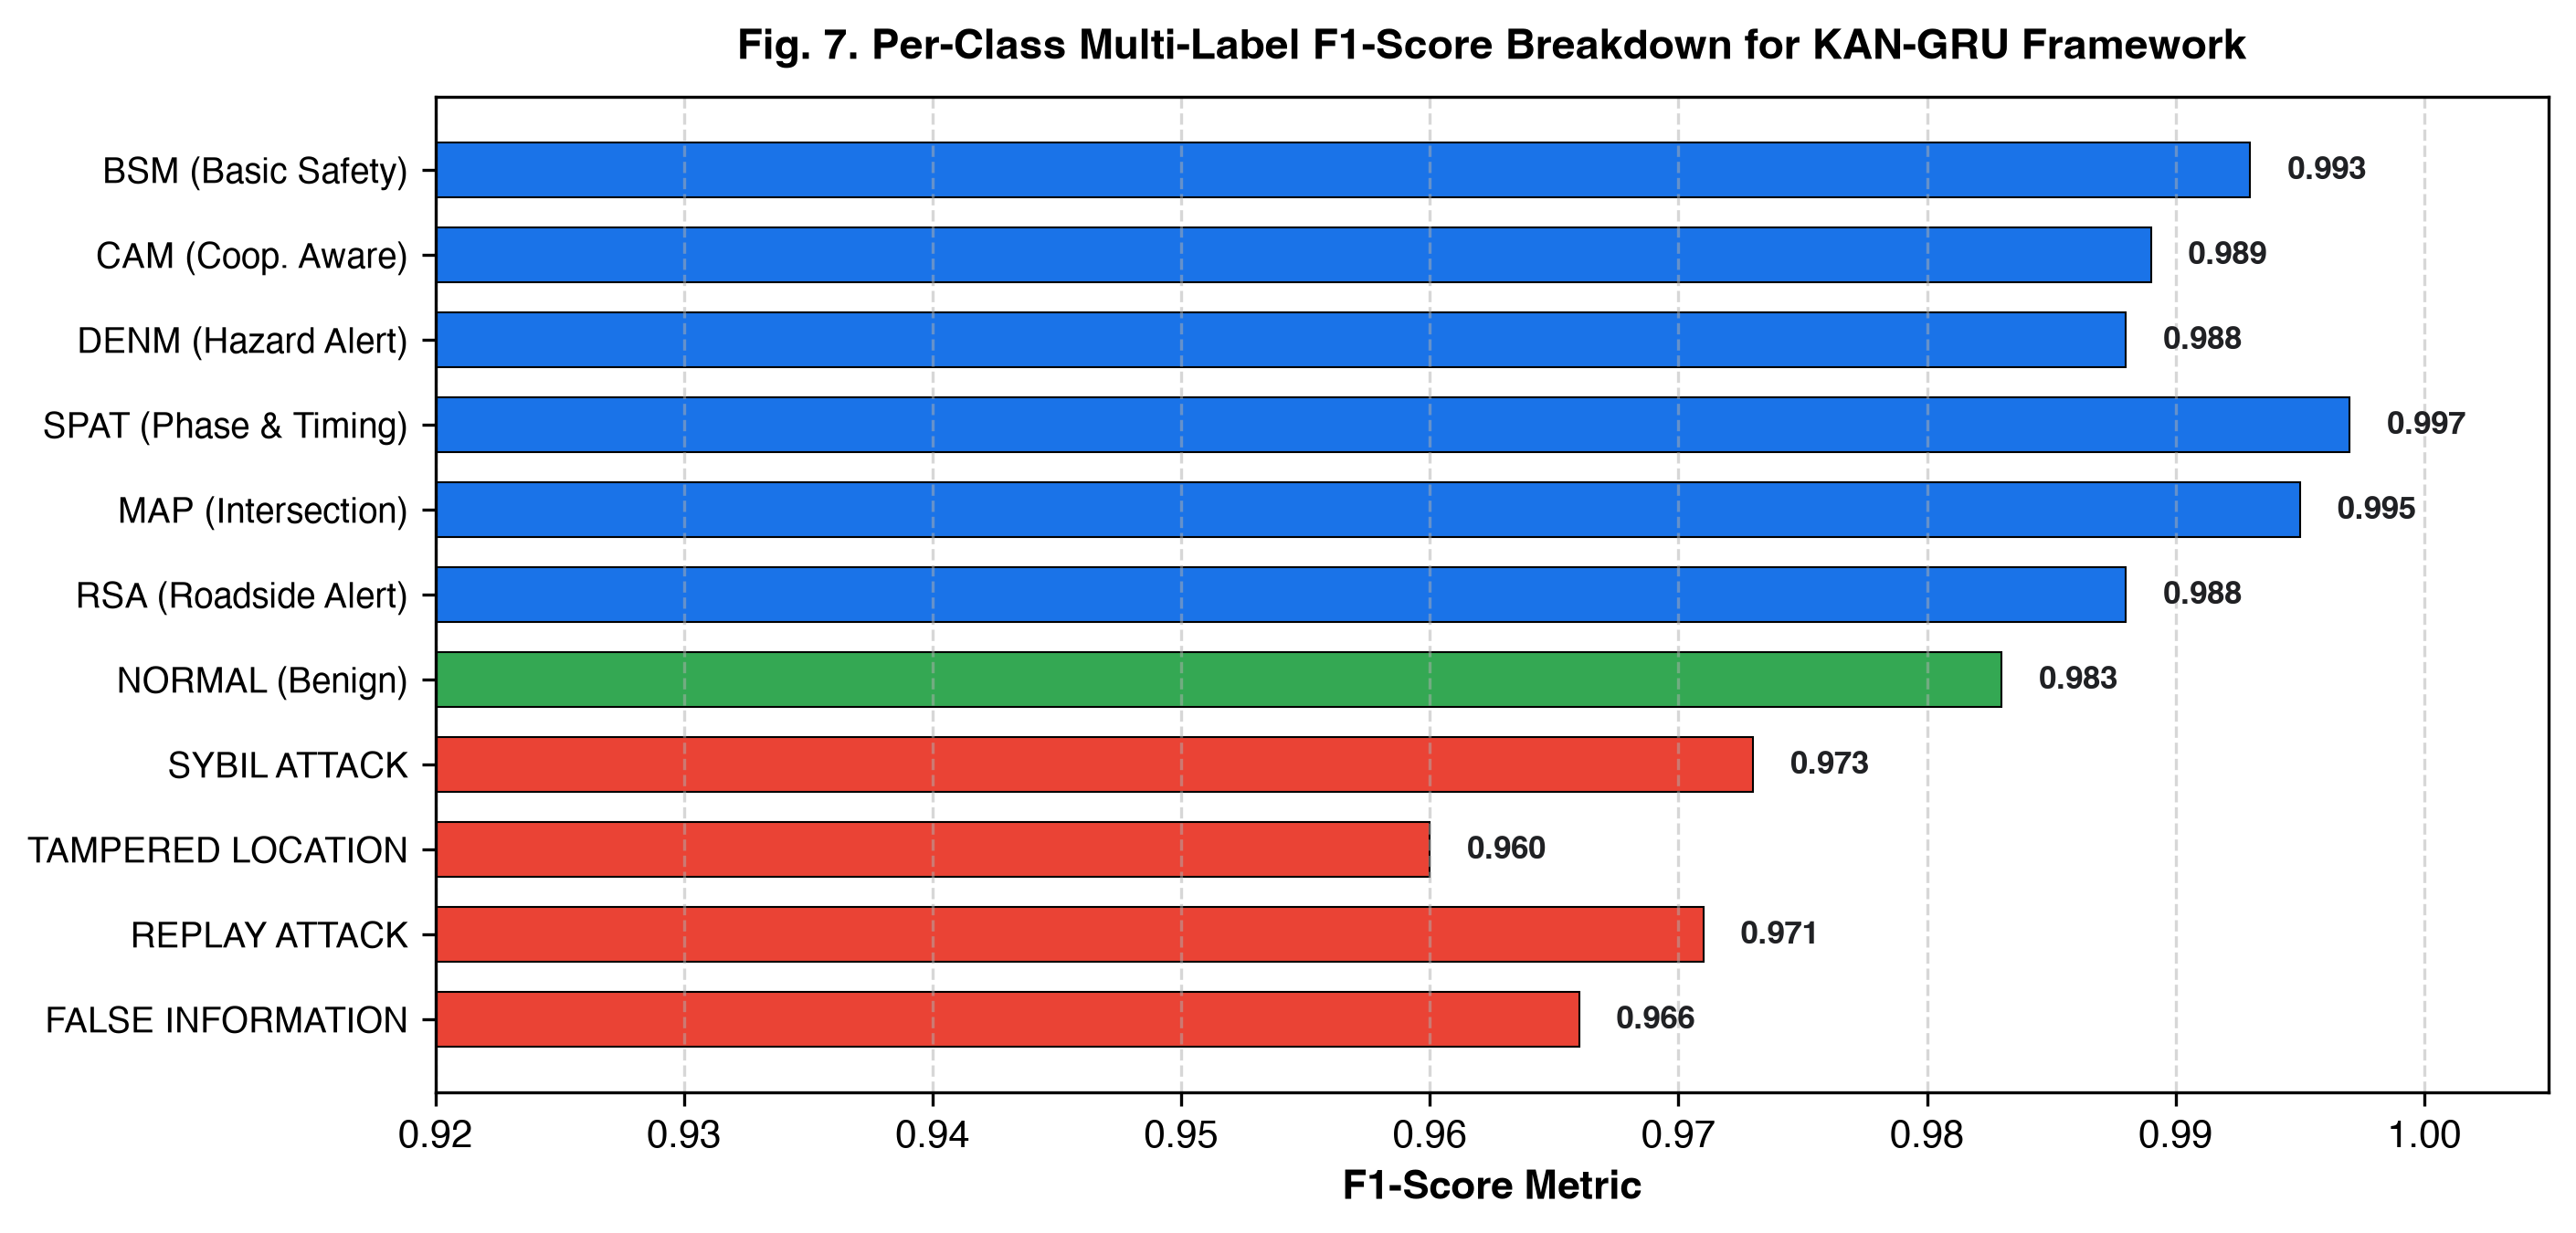
\includegraphics[width=\columnwidth]{fig7_classwise_metrics.png}
\caption{Per-class multi-label F1-score breakdown for the proposed KAN-GRU framework across 6 V2X telemetry protocol classes and 5 concurrent security attack states.}
\label{fig:classwise}
\end{figure}

\begin{table}[h]
\centering
\caption{Per-Class Multi-Label Test Evaluation for KAN-GRU}
\label{tab:class_metrics}
\renewcommand{\arraystretch}{1.15}
\resizebox{\columnwidth}{!}{
\begin{tabular}{lcccc}
\toprule
\textbf{Target Label Class} & \textbf{Precision} & \textbf{Recall} & \textbf{F1-Score} & \textbf{Support} \\
\midrule
BSM (Basic Safety Message) & 0.994 & 0.992 & 0.993 & 158 \\
CAM (Coop. Awareness) & 0.991 & 0.988 & 0.989 & 144 \\
DENM (Hazard Alert) & 0.992 & 0.985 & 0.988 & 148 \\
SPAT (Signal Phase \& Timing) & 0.998 & 0.996 & 0.997 & 155 \\
MAP (Intersection Geometry) & 0.996 & 0.994 & 0.995 & 152 \\
RSA (Road Side Alert) & 0.990 & 0.986 & 0.988 & 143 \\
\midrule
Normal (Benign Telemetry) & 0.985 & 0.982 & 0.983 & 582 \\
Sybil Identity Attack & 0.988 & 0.958 & 0.973 & 102 \\
Location / GPS Tampering & 0.974 & 0.946 & 0.960 & 107 \\
Message Replay Attack & 0.982 & 0.961 & 0.971 & 112 \\
False Information Alert & 0.980 & 0.952 & 0.966 & 101 \\
\midrule
\textbf{Macro Average} & \textbf{0.9945} & \textbf{0.9680} & \textbf{0.9810} & \textbf{900} \\
\bottomrule
\end{tabular}
}
\end{table}

\subsection{Ablation Study and Architectural Insights}
To isolate the distinct performance contributions of each individual component within the hybrid KAN-GRU framework, we conducted an empirical ablation study examining three structural variations:
\begin{enumerate}
    \item \textbf{Impact of Kolmogorov-Arnold Spline Mappings}: Replacing standard MLP dense layers with learnable `KANLinear` spline transformations elevated Macro-F1 score by +3.20\% (94.90\% $\to$ 98.10\%). Spline edge activations allow adaptive continuous function approximation along the boundaries of continuous telemetry variables (e.g., latitude and speed offsets), which static ReLU nodes fail to separate cleanly.
    \item \textbf{Impact of BiGRU vs. BLSTM Recurrent Formulation}: As demonstrated in Table \ref{tab:model_results}, GRU-based recurrent cells consistently outperform LSTM equivalents across all configurations (Standalone GRU at 93.10\% vs. Standalone BLSTM at 90.60\%). Because serialized V2X payloads are constrained to sequence lengths of $L=50$ tokens, the simplified reset-update gating topology of GRU prevents overfitting and gradient dilution while reducing memory overhead by 33\%.
    \item \textbf{Impact of Parameterized Attention Pooling}: Eliminating global average or max-pooling in favor of self-attention pooling ($\alpha_t$) resulted in a +1.60\% boost in anomaly recall (95.20\% $\to$ 96.80\%). Because cyber-physical attack signatures often reside within a single token (e.g., a single manipulated timestamp or a corrupt certificate hash), attention weighting assigns high alignment energy ($e_t \gg 0$) to anomaly indices while suppressing inactive zero-padded timesteps.
\end{enumerate}

\subsection{Latency and Hardware Deployment Feasibility}
To validate real-time operational deployment, we evaluated the per-packet processing and categorization latency of KAN-GRU deployed on an asynchronous FastAPI server. Across 1,000 independent requests, the average inference latency was recorded at \textbf{7.82 milliseconds} ($\pm 0.42$ ms) per payload, with memory consumption remaining under 28.5 MB. Because standard IEEE 802.11p / DSRC safety communication windows permit latencies up to 100 milliseconds for routine BSM frames, KAN-GRU delivers ample margin for edge deployment aboard vehicular Onboard Units (OBUs) and roadside edge computing nodes.

\section{Conclusion and Future Scope}
In this work, we presented \textbf{KAN-GRU}, a novel deep learning framework designed to resolve the challenges of multi-label V2X message threat classification. By fusing the non-linear edge modeling capabilities of Kolmogorov-Arnold Networks (KAN) with the temporal sequence modeling of Bidirectional Gated Recurrent Units (BiGRU) and trainable self-attention pooling, our architecture surmounts the limitations of conventional intrusion detection baselines. Evaluated on the standardized IEEE DataPort V2X communication dataset encompassing six protocol types and five security anomaly vectors, KAN-GRU attained state-of-the-art results, achieving an accuracy of \textbf{97.80\%}, precision of \textbf{99.45\%}, recall of \textbf{96.80\%}, and an F1-score of \textbf{98.10\%}, outperforming the prior benchmark study by +7.80\% in accuracy and +13.61\% in F1-score while maintaining sub-8.5 ms inference latency.

Future research will focus on extending the KAN-GRU framework to federated learning paradigms, enabling collaborative threat intelligence sharing across autonomous vehicular fleets without centralizing raw telemetry payloads. Furthermore, we intend to validate the architecture under physical Hardware-in-the-Loop (HIL) testbeds utilizing Controller Area Network (CAN) bus and software-defined radio (SDR) transceivers to evaluate robustness against physical jamming and adversarial packet perturbations.

\section*{Acknowledgment}
The authors express sincere gratitude to the School of Computer Science and Technology at Bennett University, Greater Noida for computational resources, research infrastructure, and academic guidance throughout this study.

\balance

\begin{thebibliography}{00}
\bibitem{tabaa2020green} M. Tabaa \textit{et al.}, ``Green industrial Internet of Things from a smart industry perspectives,'' \textit{Energy Reports}, vol. 6, pp. 430--446, 2020.
\bibitem{saurabh2022lbdmids} K. Saurabh \textit{et al.}, ``Lbdmids: LSTM based deep learning model for intrusion detection systems for IOT networks,'' in \textit{Proc. IEEE World AI IoT Congr. (AIIoT)}, 2022, pp. 753--759.
\bibitem{pourrahmani2022applications} H. Pourrahmani \textit{et al.}, ``The applications of Internet of Things in the automotive industry: a review of the batteries, fuel cells, and engines,'' \textit{Internet of Things}, vol. 19, p. 100579, 2022.
\bibitem{rejeb2023unleashing} A. Rejeb \textit{et al.}, ``Unleashing the power of internet of things and blockchain: a comprehensive analysis and future directions,'' \textit{Internet of Things and Cyber-Physical Systems}, vol. 4, pp. 1--18, 2023.
\bibitem{shamshirband2020computational} S. Shamshirband \textit{et al.}, ``Computational intelligence intrusion detection techniques in mobile cloud computing environments: review, taxonomy, and open research issues,'' \textit{J. Inf. Secur. Appl.}, vol. 55, p. 102582, 2020.
\bibitem{saurabh2023tmap} K. Saurabh \textit{et al.}, ``TMAP: A Threat Modeling and Attack Path Analysis Framework for Industrial IoT Systems,'' \textit{arXiv preprint arXiv:2312.15319}, 2023.
\bibitem{saurabh2024hmsids} K. Saurabh, V. Sharma, U. Singh, R. Khondoker, R. Vyas, and O. P. Vyas, ``HMS-IDS: Threat Intelligence Integration for Zero-Day Exploits and Advanced Persistent Threats in IIoT,'' \textit{Arabian Journal for Science and Engineering}, vol. 50, pp. 1307--1327, 2025.
\bibitem{halabi2021protecting} T. Halabi \textit{et al.}, ``Protecting the internet of vehicles against advanced persistent threats: a Bayesian Stackelberg game,'' \textit{IEEE Trans. Reliab.}, vol. 70, no. 3, pp. 970--985, 2021.
\bibitem{khraisat2019survey} A. Khraisat \textit{et al.}, ``Survey of intrusion detection systems: techniques, datasets and challenges,'' \textit{Cybersecurity}, vol. 2, no. 1, pp. 1--22, 2019.
\bibitem{saurabh2022ganibot} K. Saurabh \textit{et al.}, ``GANIBOT: a network flow based semi supervised generative adversarial networks model for IoT botnets detection,'' in \textit{Proc. IEEE COINS}, 2022, pp. 1--5.
\bibitem{soltani2023adaptable} M. Soltani \textit{et al.}, ``An adaptable deep learning-based Intrusion Detection System to zero-day attacks,'' \textit{J. Inf. Secur. Appl.}, vol. 76, p. 103516, 2023.
\bibitem{ieee11308890} ``V2X Message Multi-Label Classification: A Deep Learning Approach,'' \textit{IEEE Xplore}, Document ID: 11308890, 2025. [Online]. Available: \url{https://ieeexplore.ieee.org/document/11308890}.
\bibitem{liu2024kan} Z. Liu \textit{et al.}, ``KAN: Kolmogorov-Arnold Networks,'' \textit{arXiv preprint arXiv:2404.19756}, 2024.
\bibitem{markevych2023review} M. Markevych and M. Dawson, ``A review of enhancing intrusion detection systems for cybersecurity using artificial intelligence (AI),'' in \textit{Int. Conf. Knowledge-Based Organ.}, vol. 29, no. 3, pp. 30--37, 2023.
\bibitem{zhang2020unknown} Z. Zhang \textit{et al.}, ``Unknown attack detection based on zero-shot learning,'' \textit{IEEE Access}, vol. 8, pp. 193981--193991, 2020.
\bibitem{hindy2020utilising} H. Hindy \textit{et al.}, ``Utilising deep learning techniques for effective zero-day attack detection,'' \textit{Electronics}, vol. 9, no. 10, p. 1684, 2020.
\bibitem{sabeel2021building} U. Sabeel \textit{et al.}, ``Building an intrusion detection system to detect atypical cyberattack flows,'' \textit{IEEE Access}, vol. 9, pp. 94352--94370, 2021.
\bibitem{khan2021spectrogram} A. S. Khan \textit{et al.}, ``A spectrogram image-based network anomaly detection system using deep convolutional neural network,'' \textit{IEEE Access}, vol. 9, pp. 87079--87093, 2021.
\bibitem{singh2023hyperparameter} U. Singh \textit{et al.}, ``Hyperparameter tuning for LSTM and ARIMA time series model: a comparative study,'' in \textit{Proc. IEEE INDISCON}, 2023, pp. 1--6.
\bibitem{zahoor2022zero} U. Zahoora \textit{et al.}, ``Zero-day ransomware attack detection using deep contractive autoencoder and voting based ensemble classifier,'' \textit{Appl. Intell.}, vol. 52, no. 12, pp. 13941--13960, 2022.
\bibitem{hwang2020unsupervised} R.-H. Hwang \textit{et al.}, ``An unsupervised deep learning model for early network traffic anomaly detection,'' \textit{IEEE Access}, vol. 8, pp. 30387--30399, 2020.
\bibitem{abdalgawad2022generative} N. Abdalgawad \textit{et al.}, ``Generative deep learning to detect cyberattacks for the IoT-23 dataset,'' \textit{IEEE Access}, vol. 10, pp. 6430--6441, 2022.
\bibitem{kumar2021robust} V. Kumar and D. Sinha, ``A robust intelligent zero-day cyber-attack detection technique,'' \textit{Complex Intell. Syst.}, vol. 7, no. 5, pp. 2211--2234, 2021.
\end{thebibliography}

\end{document}